\documentclass{Academic}
\usepackage[most]{tcolorbox}

\newtcblisting{projecttreebox}{
  breakable,
  colback=black!2,
  colframe=black!35,
  boxrule=0.5pt,
  arc=2pt,
  left=6pt,
  right=6pt,
  top=6pt,
  bottom=6pt,
  listing only,
  listing options={basicstyle=\ttfamily\scriptsize},
  title=Curated Project Tree,
  fonttitle=\bfseries,
  coltitle=black
}

\newtcblisting{yamlcodebox}{
  breakable,
  colback=black!2,
  colframe=black!35,
  boxrule=0.5pt,
  arc=2pt,
  left=6pt,
  right=6pt,
  top=6pt,
  bottom=6pt,
  listing only,
  listing options={basicstyle=\ttfamily\scriptsize},
  title=Environment File (\texttt{env.yaml}),
  fonttitle=\bfseries,
  coltitle=black
}

\captionsetup[table]{skip=4pt}
\setlength{\textfloatsep}{10pt plus 2pt minus 2pt}
\setlength{\floatsep}{10pt plus 2pt minus 2pt}
\setlength{\intextsep}{10pt plus 2pt minus 2pt}

\makeatletter
\setlength{\@fptop}{0pt}
\setlength{\@fpsep}{10pt}
\setlength{\@fpbot}{0pt plus 1fil}
\makeatother

\begin{document}
%TC:ignore
\myabstract{This project develops an integrated simulation framework for Boeing 747 circular-flight tracking in a 2D plane. The framework combines: (i) a linear quadratic regulator (LQR) for heading/bank inner-loop control, (ii) a fourth-order Runge-Kutta (RK4) integrator for nonlinear aircraft dynamics stimulation, and (iii) a Gaussian Bayes/MAP estimator for state estimation under noisy measurements. Numerical experiments based on the project code show accurate path convergence and stable speed regulation, with final cross-track error close to zero and bounded bank angle throughout the simulation horizon. The report presents problem formulation, methodology, numerical results, and limitations. All LaTeX sources and Python code are openly available at \url{https://github.com/edyou25/AAE6202}.}
\renewcommand{\myTitle}{Boeing 747 Trajectory Tracking via Optimization, ODEs Solving, and State Estimation}
\renewcommand{\MyAuthor}{Yufa You$^{1}$, Ruige Yang}
\renewcommand{\MyDepartment}{Department of Aeronautical and Aviation Engineering}
\renewcommand{\MyCourse}{AAE6202 Mathematics and Computational Methods for Aviation Engineering Applications }
\renewcommand{\ID}{25144639R, 25145125R}
\renewcommand{\Keywords}{LQR, RK4, Bayesian estimation, MAP, Boeing 747, trajectory tracking}
\maketitle
\par
\onehalfspacing
%TC:endignore

\begin{figure}[!htb]
\centering
\includegraphics[width=0.62\textwidth]{../assets/747.png}
\caption{Representative Boeing 747 airframe image.}
\label{fig:b747-photo}
\end{figure}

\section{Introduction}

This project studies 2D circular trajectory tracking for a Boeing 747 model in planar flight. The goal is to build a compact workflow that combines control, simulation, and state estimation inside one framework. The implemented architecture has three core components: an LQR controller for heading and bank regulation, RK4 numerical integration for nonlinear propagation, and a Gaussian Bayes/MAP estimator for estimation diagnostics.

The overall structure of the project is also aligned with the learning objectives of AAE6202, which emphasize optimization, computational solution of differential equations, and uncertainty-aware mathematical methods for aviation engineering applications \supercite{liu2026aae6202}.

LQR is a standard optimal control method for linear systems with quadratic costs and is widely used in aerospace inner-loop design because of its predictable tuning behavior and strong stability properties \supercite{anderson1990,lewis2012,astrom2008}. For discrete-time dynamics
\[
x_{k+1}=A_d x_k + B_d u_k,
\]
the infinite-horizon LQR minimizes
\[
J=\sum_{k=0}^{\infty}\left(x_k^\top Q x_k + u_k^\top R u_k\right),
\]
with \(Q \succeq 0\) and \(R \succ 0\), leading to linear feedback \(u_k=-Kx_k\). In this project, LQR is used to stabilize heading and bank-angle errors around a circular-tracking reference.

\begin{figure}[!htb]
\centering

\includegraphics[width=0.96\textwidth]{assets/overview.png}
\caption{Interactive overview of the B747 control simulation, including the trajectory view and diagnostic telemetry panels.}
\label{fig:intro-overview}
\end{figure}

Aircraft motion remains nonlinear, so numerical integration is required. RK4 provides a practical balance between computational cost and accuracy and is commonly used for control-oriented flight simulation \supercite{hairer1993,butcher2016}. Compared with forward Euler, RK4 reduces truncation error significantly while remaining straightforward to implement.

The third component is Gaussian Bayesian estimation. Under Gaussian assumptions, a Bayes update is equivalent to a weighted MAP problem, linking estimation with uncertainty interpretation \supercite{kalman1960,simon2006,welch2006}. In the current code, the estimator is used for diagnostics rather than closed-loop feedback, but it still provides insight into innovation magnitude, covariance contraction, and posterior consistency.

\begin{figure}[!htb]
\centering
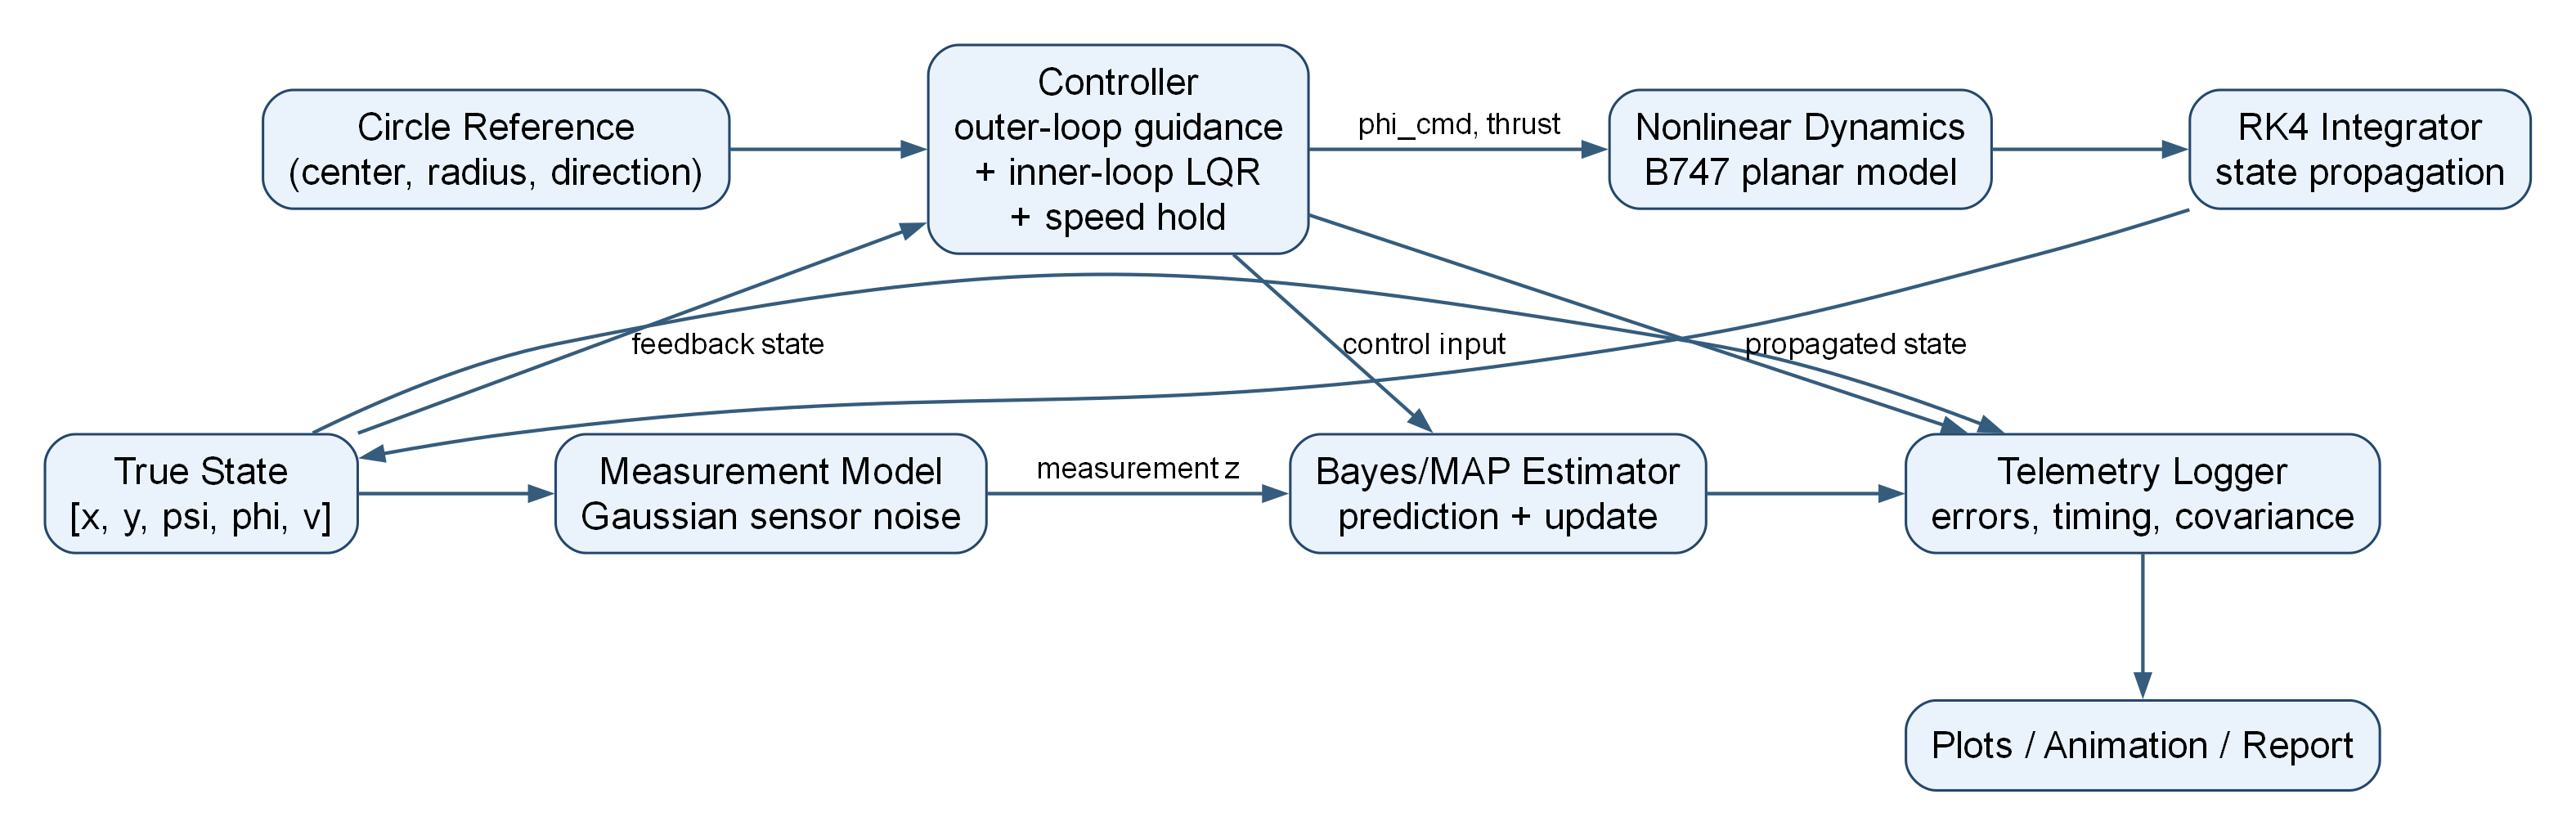
\includegraphics[width=0.99\textwidth,height=0.42\textheight,keepaspectratio]{assets/system_architecture.png}
\caption{System-level architecture of the integrated controller--simulation--estimator workflow.}
\label{fig:system-architecture}
\end{figure}

More broadly, the present work is also related to the larger optimization literature. The quadratic-cost formulation behind LQR is naturally connected to classical linear and nonlinear programming \supercite{luenberger2008}, while the tuning of state and input penalties follows the logic of convex optimization and structured tradeoff design \supercite{boyd2004}. From the viewpoint of nonlinear state evolution, the trajectory-tracking problem can also be interpreted as a controlled dynamical system whose transient and asymptotic behavior is best understood in state-space terms \supercite{scheinerman2012,dilao2023}. In addition, although the current project is not formulated as a full uncertainty-aware optimization model, its estimator and sensitivity studies connect naturally to stochastic programming, robust optimization, and distributionally robust optimization \supercite{birge1997,haneveld2020,bental2009,bertsimas2011,blanchet2024,bomze2022}.

From a computational-methods perspective, the choice of RK4 is also aligned with standard engineering numerics references, which emphasize that higher-order integration is especially valuable when nonlinear coupling accumulates long-horizon propagation error \supercite{griffiths2020}.

The main contribution of this project is the integration of these three ideas into one consistent aerospace simulation workflow. The framework demonstrates how trajectory guidance, optimal regulation, nonlinear propagation, and stochastic state estimation can be combined in a concise course project.

Figure \ref{fig:intro-overview} provides a compact visual overview of the integrated simulation environment used throughout this report.

\section{Problem Statement}

\subsection{Objective}

The objective is to design and evaluate a controller-estimator simulation system that drives a Boeing 747 model to track a circular reference trajectory in planar flight while maintaining a target speed.

\subsection{State, Input, and Reference}

The continuous state is
\[
\mathbf{x}=[x,\,y,\,\psi,\,\phi,\,v]^\top,
\]
where \(x\) and \(y\) are inertial coordinates, \(\psi\) is heading, \(\phi\) is bank angle, and \(v\) is airspeed.

The control input is
\[
\mathbf{u}=[\phi_{\mathrm{cmd}},\,T]^\top,
\]
where \(\phi_{\mathrm{cmd}}\) is the commanded bank angle and \(T\) is thrust.

The reference trajectory is a counterclockwise circle centered at \((0,0)\) with radius
\[
R=120{,}000\,\mathrm{m}.
\]
This baseline reference geometry is a simulation-design choice for the present coursework report rather than a published B747 airframe parameter.


\subsection{Performance Requirements}

The tracking system should satisfy the following requirements:
\begin{enumerate}
\item Reduce the signed cross-track error \(e_{ct}=R-r\) toward zero.
\item Keep heading and bank-angle behavior smooth and stable.
\item Maintain airspeed near \(v_{\mathrm{ref}}=210\,\mathrm{m/s}\).
\item Respect actuator and physics limits on bank angle and thrust.
\end{enumerate}

\subsection{Constraints and Assumptions}

The problem is simplified by the following assumptions:
\begin{enumerate}
\item Flight is modeled in a 2D plane.
\item Aerodynamic drag is represented by a quasi-steady model.
\item Control is updated discretely with \(\Delta t=0.05\,\mathrm{s}\), while the state dynamics are propagated continuously through numerical integration.
\item Measurement noise is Gaussian, and the estimator is used only for diagnostics in the current version.
\end{enumerate}

\section{Methodology}

\subsection{Parameter Reference}

To make the numerical setup auditable, the report distinguishes between sourced airframe parameters and simulation assumptions. Published B747-400 geometry, mass, and engine data are taken from public aerospace references, while controller gains, estimator covariances, time-step choices, and closed-loop experiment settings are declared explicitly as modeling decisions for this coursework study. Table \ref{tab:param-provenance} summarizes the provenance of the main numerical values used in the report.

\begin{table}[!htb]
\centering
\caption{The main numerical parameters used in the report.}
\label{tab:param-provenance}
\small
\setlength{\tabcolsep}{4pt}
\renewcommand{\arraystretch}{1.02}
\begin{adjustbox}{max width=\textwidth}
\begin{tabular}{@{}>{\raggedright\arraybackslash}p{0.24\textwidth} >{\raggedright\arraybackslash}p{0.28\textwidth} >{\raggedright\arraybackslash}p{0.38\textwidth}@{}}
\toprule
Parameter group & Values used in this report & Source of the values \\
\midrule
Aircraft physical model & \(m=396{,}890\,\mathrm{kg}\), \(S=510.97\,\mathrm{m}^2\), \(C_{D0}=0.022\), \(k=0.048\) & B747-400 maximum takeoff weight and installed-engine family data from Boeing; wing reference area from NASA's 747-400 PCA model; \(C_{D0}\) from MIT notes quoting Boeing drag data; \(k\) inferred from \(k=1/(\pi e AR)\) using sourced geometry and a Raymer-type span-efficiency estimate \supercite{boeing747400,burken1997,mahajan2014,raymer2018} \\
Actuation and envelope assumptions & \(\tau_\phi=2.0\,\mathrm{s}\), \(|\phi|\le35^\circ\), \(v\in[120,320]\,\mathrm{m/s}\) & Simplified simulation assumptions introduced for numerical robustness and controller design; these are not claimed as manufacturer-issued 747 limits \\
Installed thrust model & \(T\in[0,1.126\times10^6]\,\mathrm{N}\) & Based on four PW4062-class engines rated at about \(63{,}300\,\mathrm{lbf}\) each on 747-400 variants \supercite{boeing747400,pw400094guide} \\
Nominal mission setup & \(R=120{,}000\,\mathrm{m}\), \(v_{\mathrm{ref}}=210\,\mathrm{m/s}\), \(\Delta t=0.05\,\mathrm{s}\), \(t_{end}=800\,\mathrm{s}\) & Coursework simulation choices for the baseline circular-tracking experiment \\
Initial condition & \([R+2000,0,96^\circ,0^\circ,210]\) & Deliberate off-circle initial condition chosen to create a visible convergence transient \\
Controller tuning & \(Q=\operatorname{diag}(30,10)\), \(R=[1]\), \(k_v=120000\), \(k_{ct}=1/3500\), heading-correction clip \(=\pm25^\circ\) & Project controller-design choices for the nominal case study \\
Estimator covariances & Process std \((2,2,0.2^\circ,0.2^\circ,0.5)\), measurement std \((40,40,1^\circ,1^\circ,2)\), initial std \((50,50,2^\circ,2^\circ,3)\) & Project estimator settings for diagnostic uncertainty visualization \\
Sensitivity sweeps & \(\Delta t\in\{0.02,0.05,0.10,0.20\}\,\mathrm{s}\), \(R\in\{80,120,160,200\}\,\mathrm{km}\), noise scale \(\in\{0.5,1,2,4\}\), three LQR weight sets & Experiment-design choices for robustness and sensitivity analysis \\
RK4/Euler benchmark & \(\Delta t_{\mathrm{ref}}=0.05\,\mathrm{s}\), \(\Delta t_{\mathrm{test}}=0.5\,\mathrm{s}\), \(T_{\mathrm{sim}}=100\,\mathrm{s}\), \(\phi_{\mathrm{cmd}}=15^\circ+10^\circ\sin(2\pi t/20)\) & Independent numerical benchmark settings chosen to compare integrators under oscillatory bank input \\
\bottomrule
\end{tabular}
\end{adjustbox}
\end{table}

\subsection{Nonlinear B747 Planar Dynamics}

From \texttt{dynamics.py}, the planar model is
\[
\dot x = v\cos\psi,\qquad
\dot y = v\sin\psi,
\]
\[
\dot\psi = \frac{g\tan\phi}{v},\qquad
\dot\phi = \frac{\phi_{\mathrm{cmd}}-\phi}{\tau_\phi},\qquad
\dot v = \frac{T-D}{m}.
\]

The aerodynamic drag model is
\[
D=\frac12 \rho v^2 S C_D,\qquad
C_D=C_{D0}+k C_L^2,\qquad
C_L=\frac{2mg}{\rho v^2 S \cos\phi}.
\]
This particular planar B747 parameterization combines published 747-400 airframe data with standard aerodynamic approximations. The mass is set to the public 747-400 maximum takeoff weight, the wing area follows the NASA 747-400 PCA benchmark model, the parasitic drag coefficient uses the widely quoted \(C_{D0}\approx0.022\) for the Boeing 747, and the induced-drag factor is estimated from standard drag-polar relations using the sourced wing geometry \supercite{boeing747400,burken1997,mahajan2014,raymer2018}.

Key parameters from \texttt{B747Params} are:
\begin{enumerate}
\item \(m=396{,}890\,\mathrm{kg}\), \(S=510.97\,\mathrm{m}^2\)
\item \(C_{D0}=0.022\), \(k=0.048\)
\item \(\tau_\phi=2.0\,\mathrm{s}\)
\item \(|\phi|\le35^\circ\), \(T\in[0,\,1.126\times10^6]\,\mathrm{N}\)
\item \(v\in[120,\,320]\,\mathrm{m/s}\) with safety clipping
\end{enumerate}
The first two entries are directly sourced from public B747-400 references, the drag coefficients are sourced or inferred from standard aerodynamic references as described above, and the roll time constant plus clipping bounds remain simulation assumptions adopted for numerical robustness in the current project \supercite{boeing747400,burken1997,mahajan2014,raymer2018,pw400094guide}.

\subsection{RK4 Discretization}

For each simulation step, with constant input over \([t_k,t_{k+1}]\), RK4 evaluates
\[
k_1=f(x_k,u_k),\qquad
k_2=f\left(x_k+\frac{\Delta t}{2}k_1,u_k\right),
\]
\[
k_3=f\left(x_k+\frac{\Delta t}{2}k_2,u_k\right),\qquad
k_4=f\left(x_k+\Delta t\,k_3,u_k\right),
\]
and updates the state by
\[
x_{k+1}=x_k+\frac{\Delta t}{6}(k_1+2k_2+2k_3+k_4).
\]

The supplementary benchmark materials are consistent with this RK4 modeling idea in the sense that they use the same five-dimensional state \([x,y,\psi,\phi,v]\), the same drag construction based on \(C_L\) and \(C_D\), and a direct comparison between RK4 and forward Euler under identical control inputs. In the final report, however, the cited physical parameter values are taken from public aerospace references rather than from local code files.

\subsection{Circular Tracking Controller}

From \texttt{controller.py}, the controller has three layers.

First, an outer-loop geometry-based guidance law computes current radius, circle tangent heading, and signed cross-track error. A bounded heading correction is added:
\[
\psi_{\mathrm{des}}=\psi_{\mathrm{tangent}}+\operatorname{clip}\left(\arctan\left(k_{ct}(-e_{ct})\right),\pm25^\circ\right).
\]

Second, a feedforward bank command for circular motion is generated from
\[
\phi_{ff}=\arctan\left(\frac{v_{\mathrm{ref}}^2}{gR}\right),
\]
with the correct sign for the direction of turn and with saturation at the bank-angle limit.

Third, an inner-loop LQR regulates heading and bank-angle errors,
\[
e_\psi=\psi-\psi_{\mathrm{des}},\qquad e_\phi=\phi-\phi_{ff}.
\]
Using the linearized error dynamics
\[
\dot e_\psi=\frac{g}{v_{\mathrm{ref}}}e_\phi,\qquad
\dot e_\phi=-\frac{1}{\tau_\phi}e_\phi+\frac{1}{\tau_\phi}u,
\]
where \(u=\Delta\phi_{\mathrm{cmd}}\), the code forms a discrete approximation
\[
A_d\approx I+\Delta tA,\qquad B_d\approx \Delta tB,
\]
solves the discrete Riccati equation, and applies
\[
\Delta\phi_{\mathrm{cmd}}=-K[e_\psi,\,e_\phi]^\top,\qquad
\phi_{\mathrm{cmd}}=\phi_{ff}+\Delta\phi_{\mathrm{cmd}}.
\]

The speed loop uses
\[
T = D_{\mathrm{guess}} + k_v(v_{\mathrm{ref}}-v),
\]
followed by clipping to thrust bounds.
The feedforward-turn formula comes from coordinated-turn kinematics, while the numerical values \(k_v=120000\), \(k_{ct}=1/3500\), and the \(\pm25^\circ\) heading-correction clip are baseline controller-tuning choices for this case study \supercite{astrom2008}.

Default LQR weighting in \texttt{ControlConfig} is
\[
Q=\operatorname{diag}(30,\,10),\qquad R=[1].
\]
These weights are not taken from a handbook table; they are the baseline tuning adopted for the nominal simulation and the later sensitivity study.

\begin{figure}[!htb]
\centering
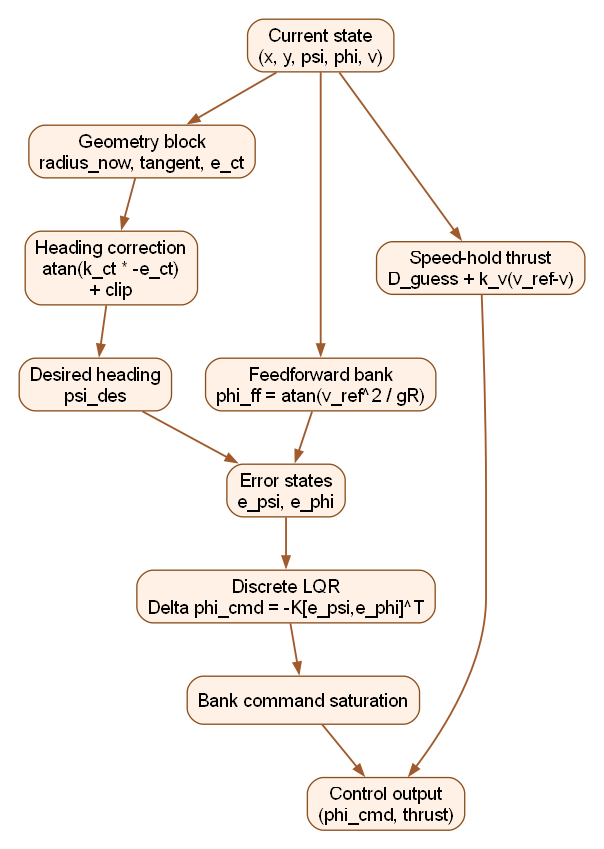
\includegraphics[width=0.50\textwidth]{assets/controller_logic.png}
\caption{Detailed control-logic flow from geometric error to saturated command output.}
\label{fig:controller-logic}
\end{figure}

Figure \ref{fig:controller-logic} makes the layered design explicit. Geometric guidance computes the desired heading, coordinated-turn physics provides a feedforward bank angle, and LQR then stabilizes the residual angular errors. This decomposition is easier to interpret and tune than a monolithic controller, which is one reason it works well in an educational setting.

\subsection{Gaussian Bayes/MAP Estimator}

From \texttt{estimation.py}, the estimator performs prediction, update, and MAP diagnostics.

Prediction:
\[
x_k^- = f_{RK4}(x_{k-1}^+,u_{k-1}),\qquad
P_k^- = P_{k-1}^+ + Q.
\]

Update:
\[
K_k=P_k^-(P_k^-+R)^{-1},
\]
\[
x_k^+=x_k^-+K_k(z_k-x_k^-),\qquad
P_k^+=(I-K_k)P_k^-.
\]

The MAP objective evaluated at the posterior state is
\[
\mathcal{L}_{MAP}
=\frac12(x_k^+-x_k^-)^\top(P_k^-)^{-1}(x_k^+-x_k^-)
+\frac12(z_k-x_k^+)^\top R^{-1}(z_k-x_k^+).
\]

The noise settings are:
\begin{enumerate}
\item Process standard deviation: \((2,\,2,\,0.2^\circ,\,0.2^\circ,\,0.5)\)
\item Measurement standard deviation: \((40,\,40,\,1^\circ,\,1^\circ,\,2)\)
\item Initial standard deviation: \((50,\,50,\,2^\circ,\,2^\circ,\,3)\)
\end{enumerate}
These covariance surrogates are project-level estimator settings for diagnostic visualization rather than quantities identified from flight-test data.

\subsection{Simulation Workflow}

At each simulation step in \texttt{run.py}, the following sequence is executed:
\begin{enumerate}
\item Compute control action and control diagnostics.
\item Generate a noisy measurement.
\item Run the estimator update.
\item Propagate the true state with RK4.
\item Log telemetry for analysis and visualization.
\end{enumerate}

\subsection{Software Architecture and Data Flow}

From a software-engineering perspective, the project is organized as a compact closed-loop pipeline. The geometric reference is supplied to the controller, the controller generates bank-angle and thrust commands, the nonlinear B747 dynamics are propagated by RK4, and noisy measurements are processed by the Gaussian Bayes/MAP estimator. At the same time, telemetry signals such as tracking errors, timing, innovation norms, covariance traces, and state derivatives are collected for post-processing and report generation. This structure is intentionally modular: each mathematical part of the coursework corresponds directly to one code module.

For reproducibility, the implementation structure is also summarized through a curated project tree. The root directory contains the main simulation modules, including controller design, nonlinear dynamics, estimation, reporting, visualization, and the executable entry point. The \texttt{tests/} folder stores unit tests for each functional module. The \texttt{docs/} folder contains the written technical notes and report drafts. The \texttt{data/} folder stores runtime animations, summary metrics, and test outputs. The \texttt{latex/} folder contains the final report source, bibliography, class file, compiled PDF artifacts, and a dedicated \texttt{assets/} directory that centralizes every Python-generated figure and Graphviz source referenced by the manuscript.

\begin{projecttreebox}
AAE6202
|-- controller.py
|-- dynamics.py
|-- estimation.py
|-- reporting.py
|-- extended_reporting.py
|-- run.py
|-- visual.py
|-- env.yaml
|-- README.md
|-- README_en.md
|-- assets
|   |-- 747.png
|   \-- ...
|-- data
|   |-- circle_flight_animation.gif
|   |-- report_ext
|   |   \-- report_metrics.json
|   \-- test_outputs
|-- docs
|   |-- estimation.md
|   |-- lqr.md
|   |-- project_report.md
|   |-- rk.md
|   |-- unit_test_report.md
|-- latex
|   |-- abstract.tex
|   |-- Academic.cls
|   |-- references.bib
|   |-- wordcount.py
|   |-- _main.tex
|   |-- assets
|   |   |-- controller_logic.dot
|   |   |-- controller_logic.png
|   |   |-- dt_sensitivity.png
|   |   \-- ...
|   |-- output
|   |   |-- _main-words.tex
|   |   \-- _main.pdf
|   \-- template
|       |-- abstract.tex
|       |-- Academic.cls
|       |-- references.bib
|       \-- _main.tex
|-- tests
|   |-- test_controller.py
|   |-- test_dynamics.py
|   |-- test_estimation.py
|   |-- test_eular_rk.py
|   |-- test_reporting.py
|   |-- test_run.py
|   \-- test_visual.py
\-- .git
\end{projecttreebox}


Figure \ref{fig:system-architecture} emphasizes that the controller and estimator use the same dynamic context but serve different roles. The controller shapes trajectory-tracking behavior, whereas the estimator is currently diagnostic and does not yet close the feedback loop. This separation is useful in a course project because it allows control performance and estimation behavior to be studied independently before tighter integration is attempted.

\begin{yamlcodebox}
name: aae6202
channels:
  - conda-forge
  - defaults
dependencies:
  - python=3.11
  - numpy
  - matplotlib
  - pillow
  - pip
\end{yamlcodebox}



\section{Results}

\subsection{Experiment Setup}

The baseline case in \texttt{run.py} uses \(t_{end}=800\,\mathrm{s}\), \(\Delta t=0.05\,\mathrm{s}\) (16{,}000 steps), initial state \([x_0,y_0,\psi_0,\phi_0,v_0]=[R+2000,\,0,\,96^\circ,\,0^\circ,\,210]\), and random seed 6202 for measurement noise. Figures and tables are generated automatically from the project code and exported to \texttt{latex/assets/}.

\subsection{Tracking and Regulation Performance}

Table \ref{tab:tracking-metrics} reports the nominal closed-loop metrics.

\begin{table}[!htb]
\centering
\caption{Tracking and regulation performance metrics}
\label{tab:tracking-metrics}
\small
\setlength{\tabcolsep}{4pt}
\renewcommand{\arraystretch}{0.96}
\begin{tabular}{@{}lr@{}}
\toprule
Metric & Value \\
\midrule
Final signed cross-track error \(e_{ct}\) & \(0.218\,\mathrm{m}\) \\
Final \(|e_{ct}|\) & \(0.218\,\mathrm{m}\) \\
Overall RMSE of \(e_{ct}\) (0--800 s) & \(269.24\,\mathrm{m}\) \\
MAE of \(e_{ct}\) & \(60.64\,\mathrm{m}\) \\
RMSE of \(e_{ct}\) (100--800 s) & \(5.56\,\mathrm{m}\) \\
Settling time to \(|e_{ct}|<500\,\mathrm{m}\) & \(27.8\,\mathrm{s}\) \\
Settling time to \(|e_{ct}|<100\,\mathrm{m}\) & \(78.35\,\mathrm{s}\) \\
Heading error RMSE & \(2.31^\circ\) \\
Max \(|\phi|\) & \(27.67^\circ\) \\
Max \(|\phi_{\mathrm{cmd}}|\) & \(35.0^\circ\) \\
Command saturation ratio & \(0.356\%\) \\
Mean speed & \(209.724\,\mathrm{m/s}\) \\
Speed RMSE to \(v_{\mathrm{ref}}=210\) & \(0.276\,\mathrm{m/s}\) \\
\bottomrule
\end{tabular}
\end{table}

The overall cross-track RMSE is dominated by the intentional initial offset, but after the transient the residual radial error is small. Bank angle remains within limits, command saturation is rare, and speed tracking stays tight around \(210\,\mathrm{m/s}\).

\begin{figure}[!htb]
\centering
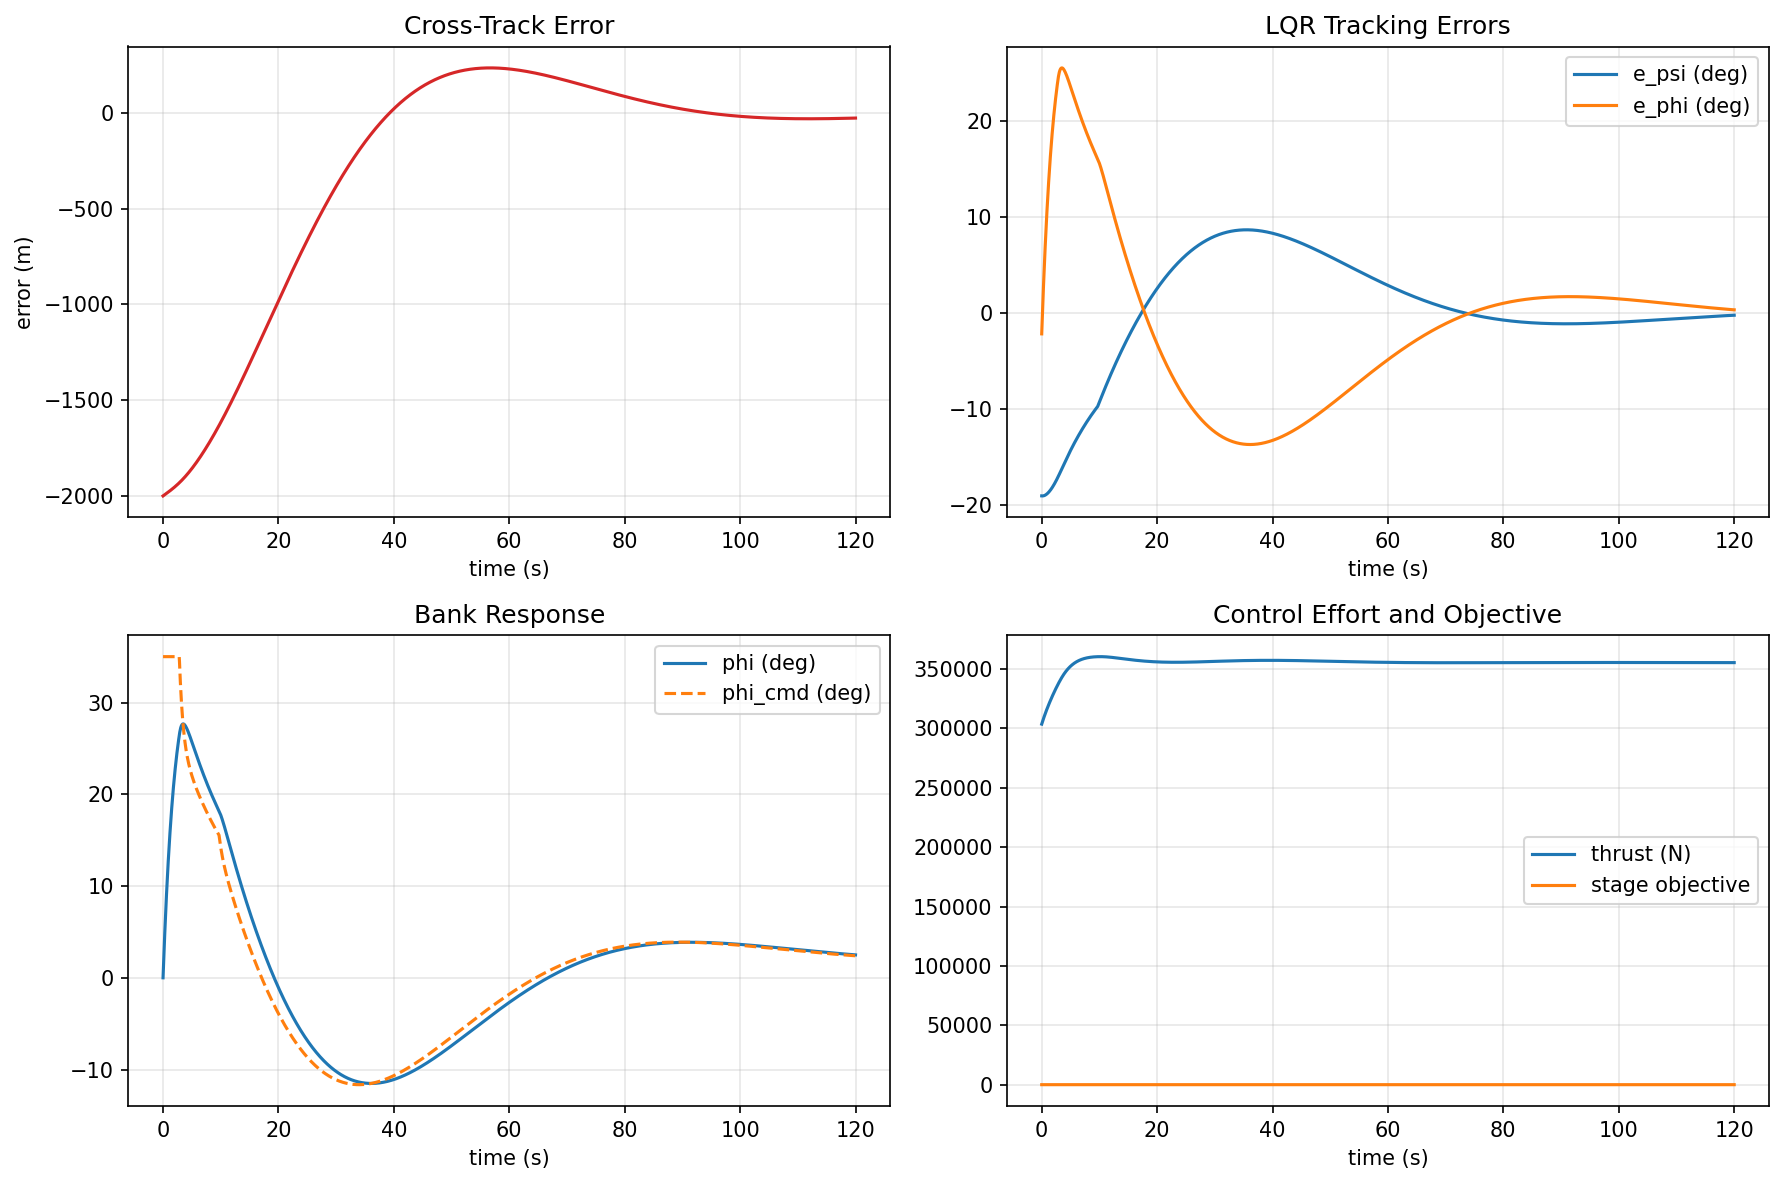
\includegraphics[width=0.93\textwidth]{assets/part1_control.png}
\caption{Detailed control figure: tracking errors, bank response, and control effort in the nominal case.}
\label{fig:appendix-part1}
\end{figure}

Figure \ref{fig:appendix-part1} confirms smooth decay of the tracking errors, close agreement between commanded and realized bank angle, and well-behaved thrust demand.

\subsection{Computational Efficiency}

Table \ref{tab:timing-metrics} shows controller and estimator timing.

\begin{table}[!htb]
\centering
\caption{Computation time metrics}
\label{tab:timing-metrics}
\small
\setlength{\tabcolsep}{4pt}
\renewcommand{\arraystretch}{0.96}
\begin{tabular}{@{}lr@{}}
\toprule
Metric & Value \\
\midrule
Mean controller computation time & \(0.0165\,\mathrm{ms}\) \\
95th percentile controller time & \(0.0176\,\mathrm{ms}\) \\
Mean estimator update time & \(0.0344\,\mathrm{ms}\) \\
95th percentile estimator time & \(0.0365\,\mathrm{ms}\) \\
\bottomrule
\end{tabular}
\end{table}

Both runtimes are negligible relative to the \(50\,\mathrm{ms}\) control interval, so the framework is comfortably fast enough for the present simulation setting.

\begin{figure}[!htb]
\centering
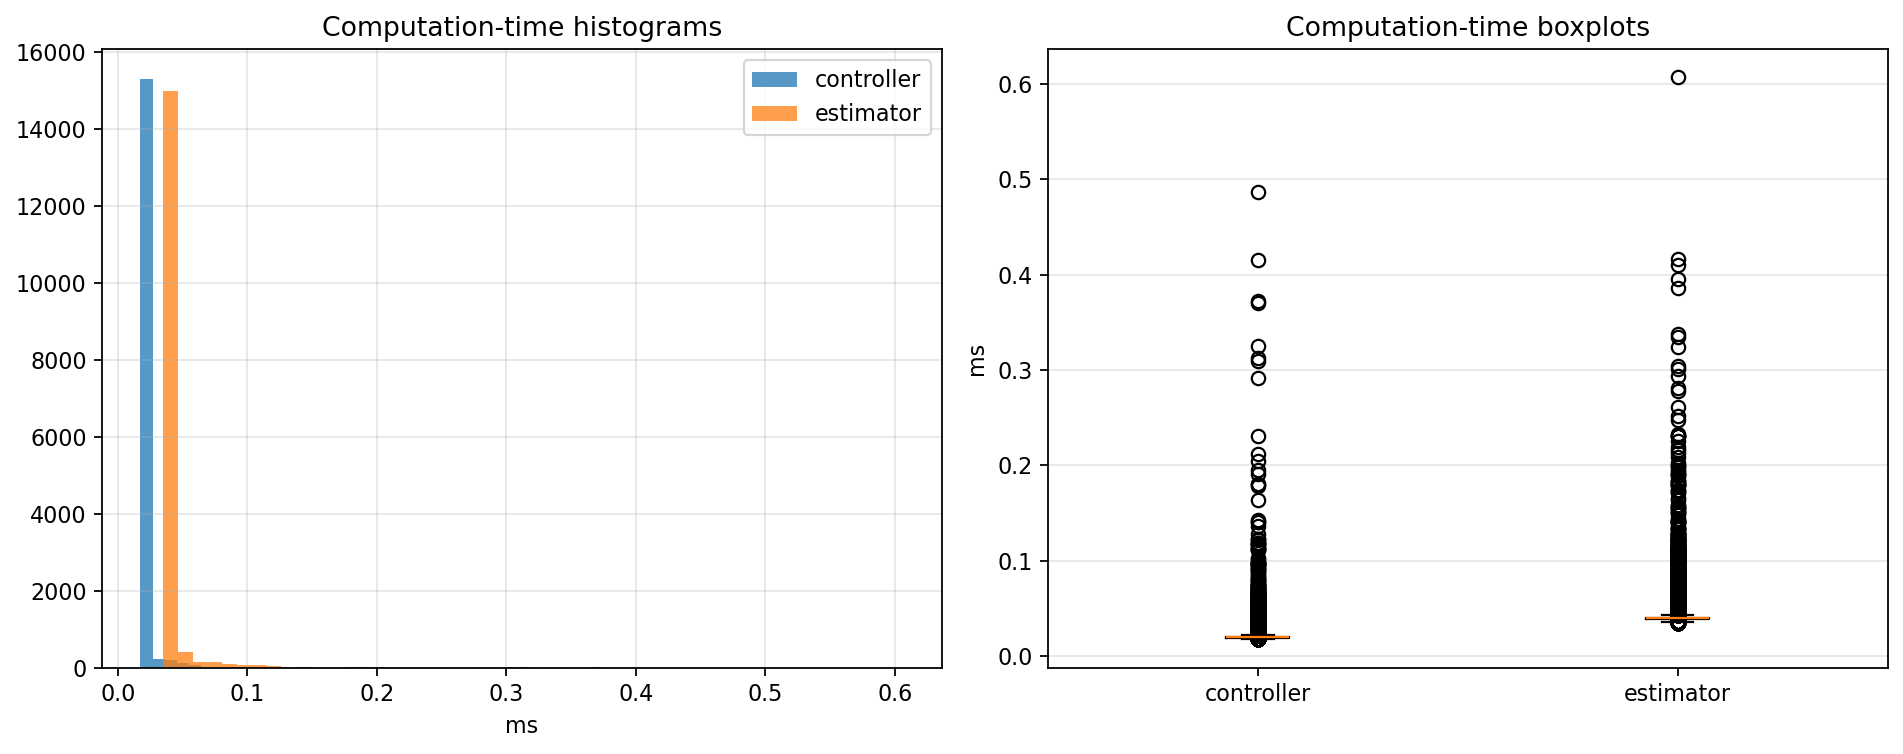
\includegraphics[width=0.93\textwidth]{assets/timing_distribution.png}
\caption{Distribution of controller and estimator computation times.}
\label{fig:timing-distribution}
\end{figure}

Figure \ref{fig:timing-distribution} shows that the timing distributions are compact and do not exhibit problematic long tails.

\subsection{Estimation Diagnostics}

Table \ref{tab:estimation-metrics} summarizes the nominal estimation statistics.

\begin{table}[!htb]
\centering
\caption{Estimator diagnostic metrics}
\label{tab:estimation-metrics}
\small
\setlength{\tabcolsep}{4pt}
\renewcommand{\arraystretch}{0.96}
\begin{tabular}{@{}lr@{}}
\toprule
Metric & Value \\
\midrule
Mean prior error norm \(\lVert x^- - x\rVert\) & \(8.380\) \\
Mean posterior error norm \(\lVert x^+ - x\rVert\) & \(8.379\) \\
Fraction of steps where posterior improves error & \(50.62\%\) \\
Mean innovation norm \(\lVert z-x^-\rVert\) & \(50.67\) \\
Mean trace reduction \(\mathrm{tr}(P^-)\rightarrow\mathrm{tr}(P^+)\) & \(5.15\%\) \\
\bottomrule
\end{tabular}
\end{table}

The covariance contracts after each update, but the posterior mean improves only slightly over the prior because process and measurement uncertainties are of similar scale. Since the controller still uses the true state, these results mainly quantify estimator consistency rather than closed-loop benefit.

\begin{figure}[!htb]
\centering
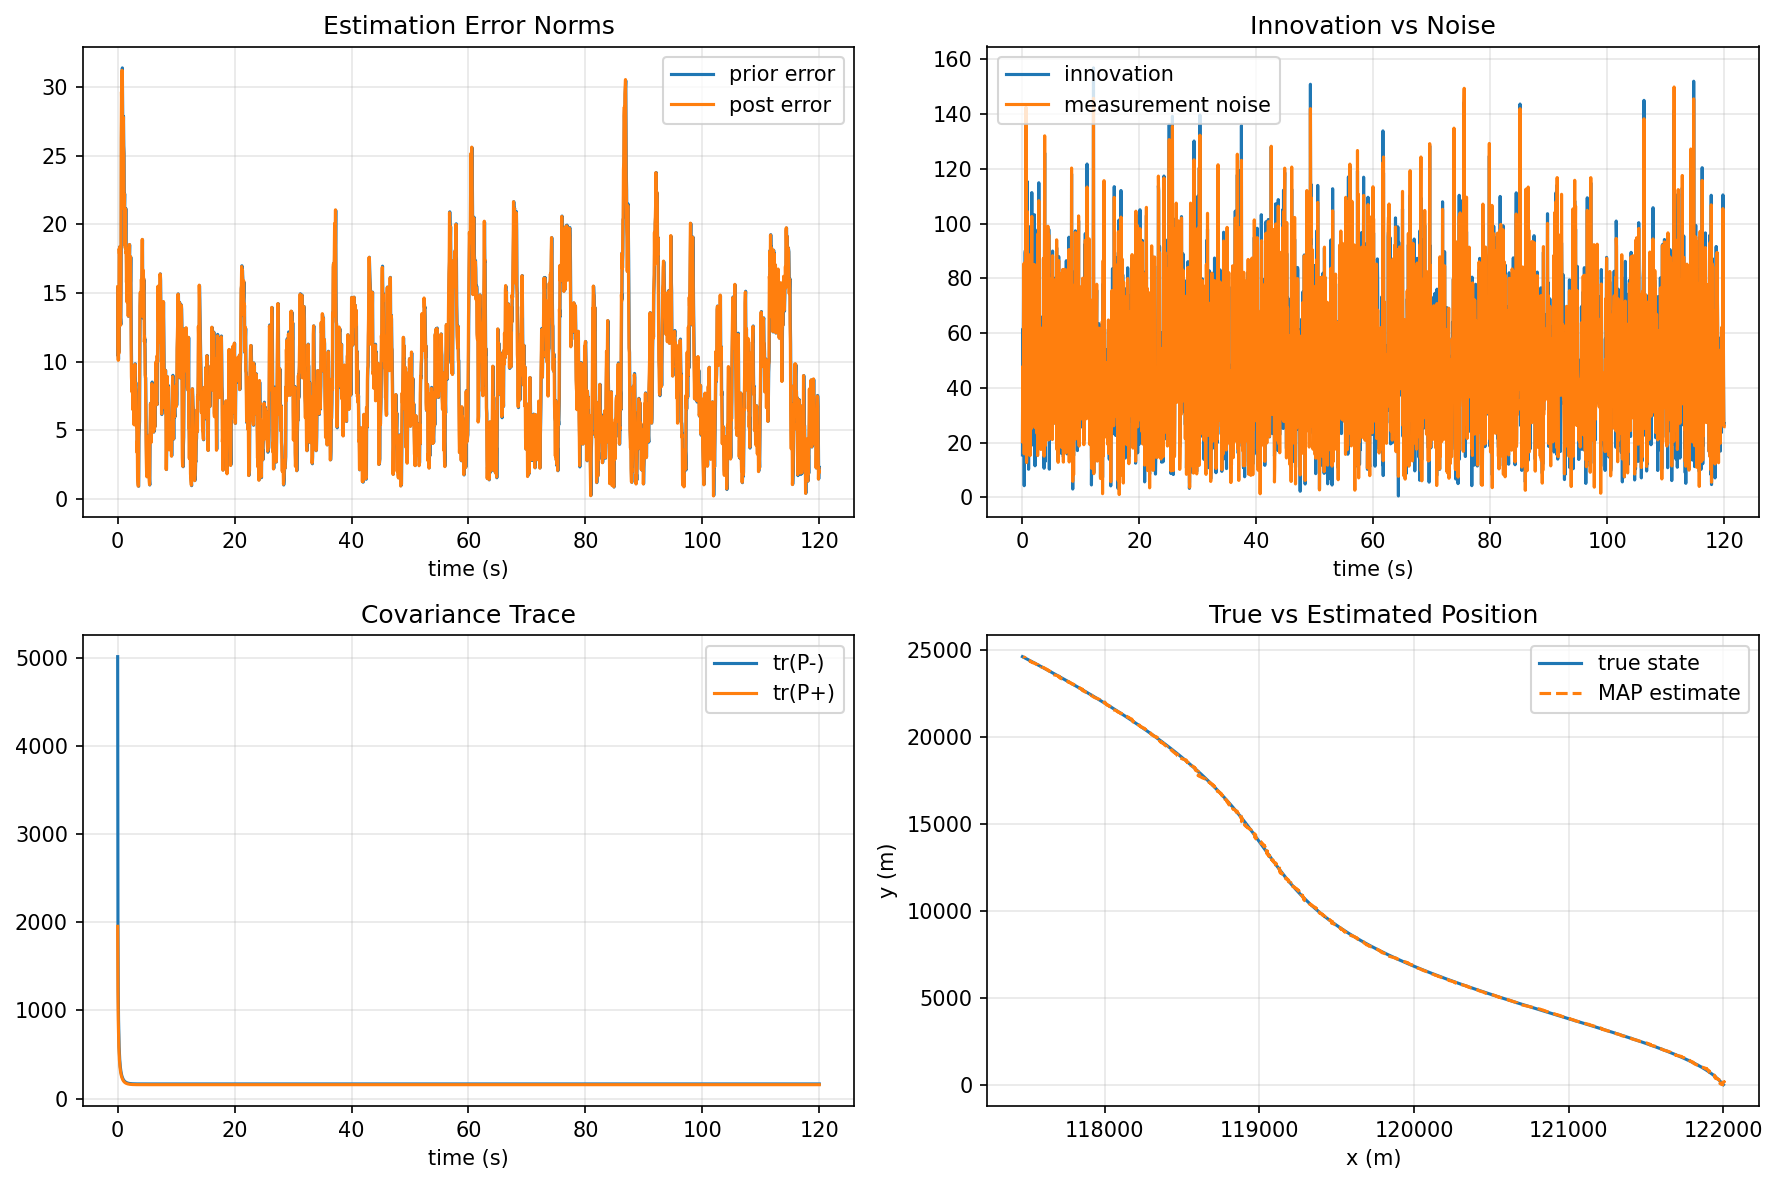
\includegraphics[width=0.93\textwidth]{assets/part3_estimation.png}
\caption{Compact estimation summary: error norms, innovation, covariance trace, and true-versus-estimated position.}
\label{fig:appendix-part3}
\end{figure}

Figure \ref{fig:appendix-part3} visualizes prior/posterior errors, innovation magnitude, covariance reduction, and estimated versus true position in the nominal case.

\begin{figure}[!htb]
\centering
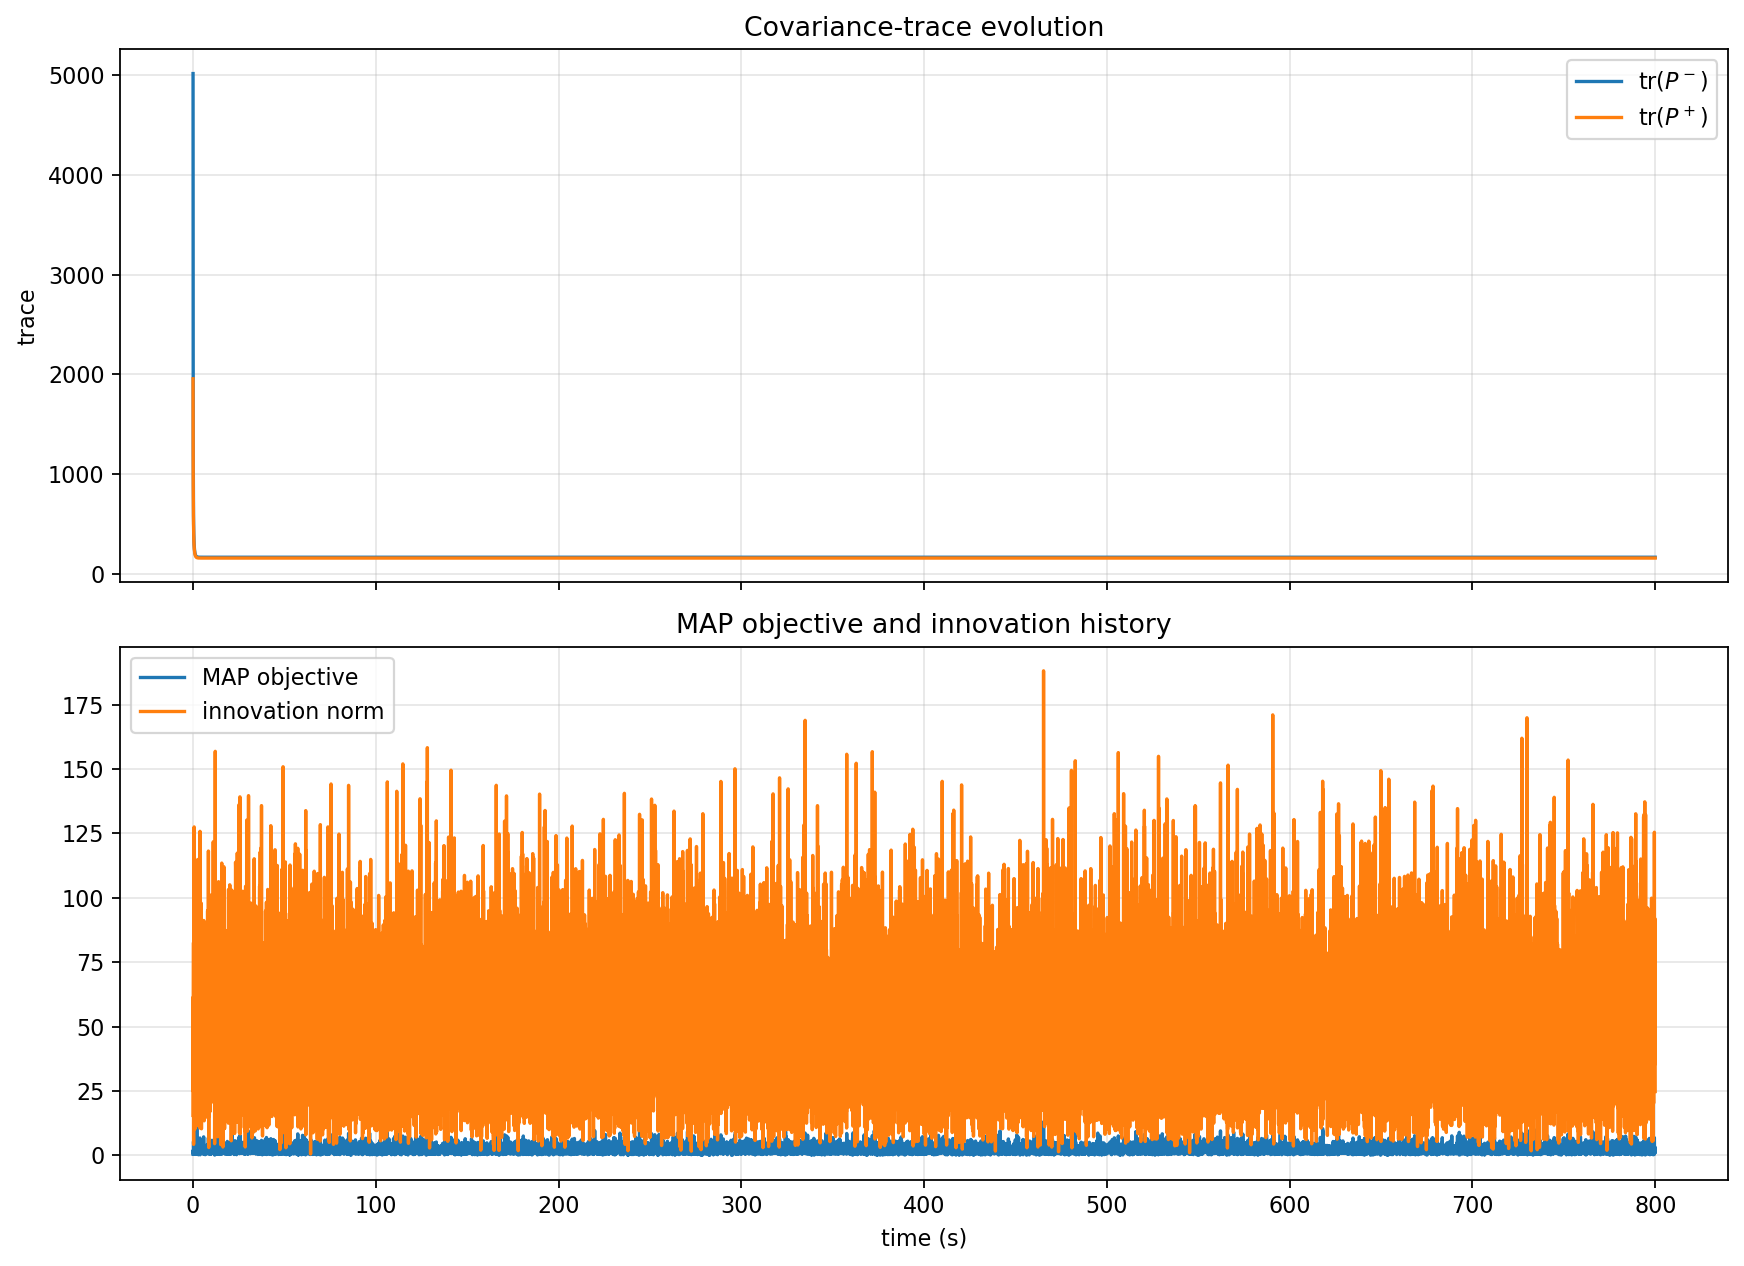
\includegraphics[width=0.93\textwidth]{assets/estimation_covariance_detail.png}
\caption{Detailed estimation diagnostics: covariance traces, MAP objective, and innovation history.}
\label{fig:estimation-covariance-detail}
\end{figure}

Figure \ref{fig:estimation-covariance-detail} adds the covariance-trace and MAP-objective detail behind the scalar estimator metrics.

\subsection{Trajectory and State Histories}

The baseline trajectory starts outside the target circle and converges smoothly to stable circular motion. The heading, bank-angle, and speed states remain bounded and physically reasonable throughout the run.

\begin{figure}[!htb]
\centering
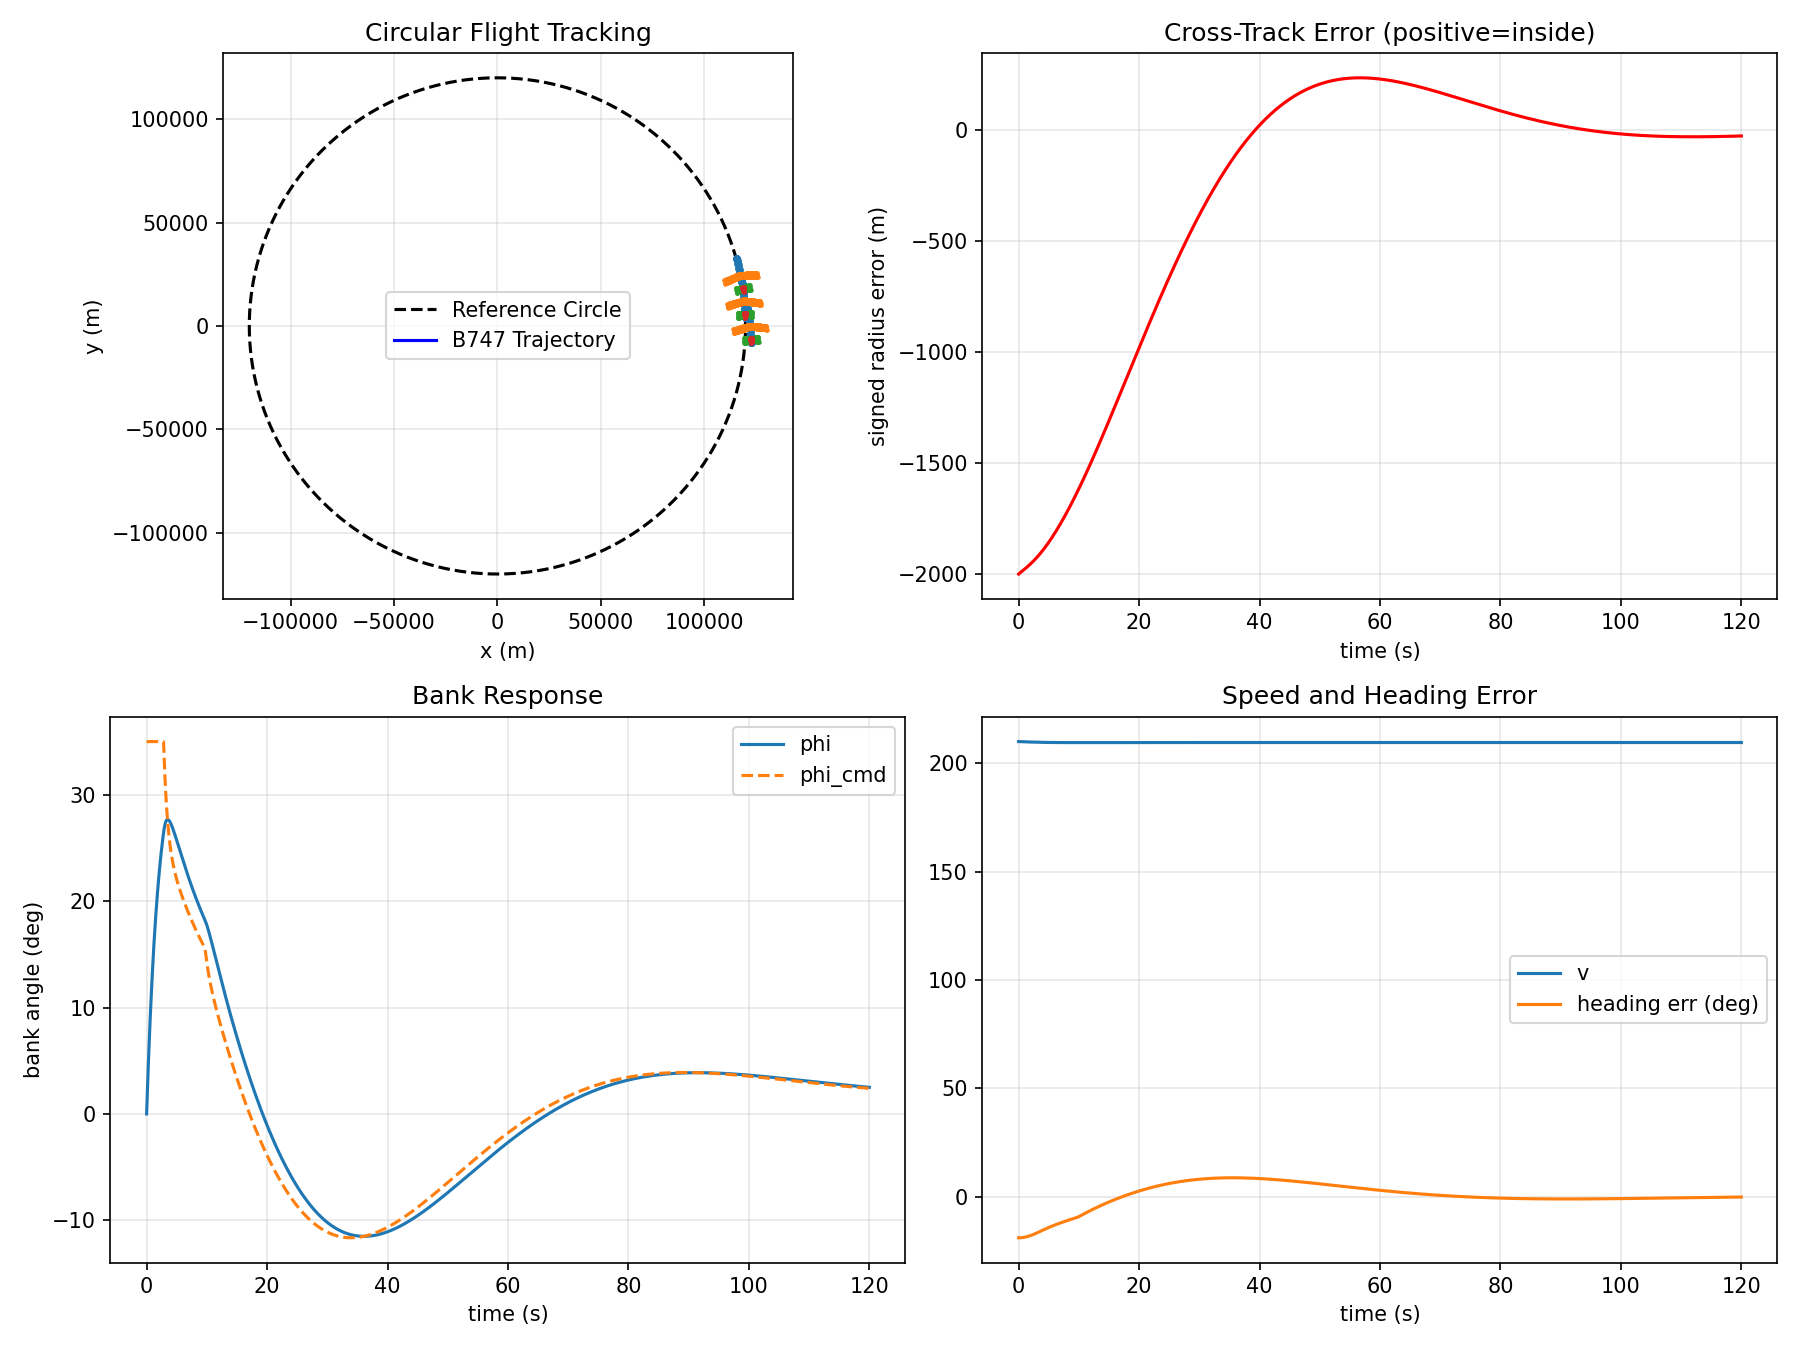
\includegraphics[width=0.9\textwidth]{assets/simulation_overview.png}
\caption{Overview of circular tracking performance generated from the project code.}
\label{fig:overview}
\end{figure}

Figure \ref{fig:overview} provides a compact global view of the nominal closed-loop behavior before the detailed state plots are examined.

\begin{figure}[!htb]
\centering
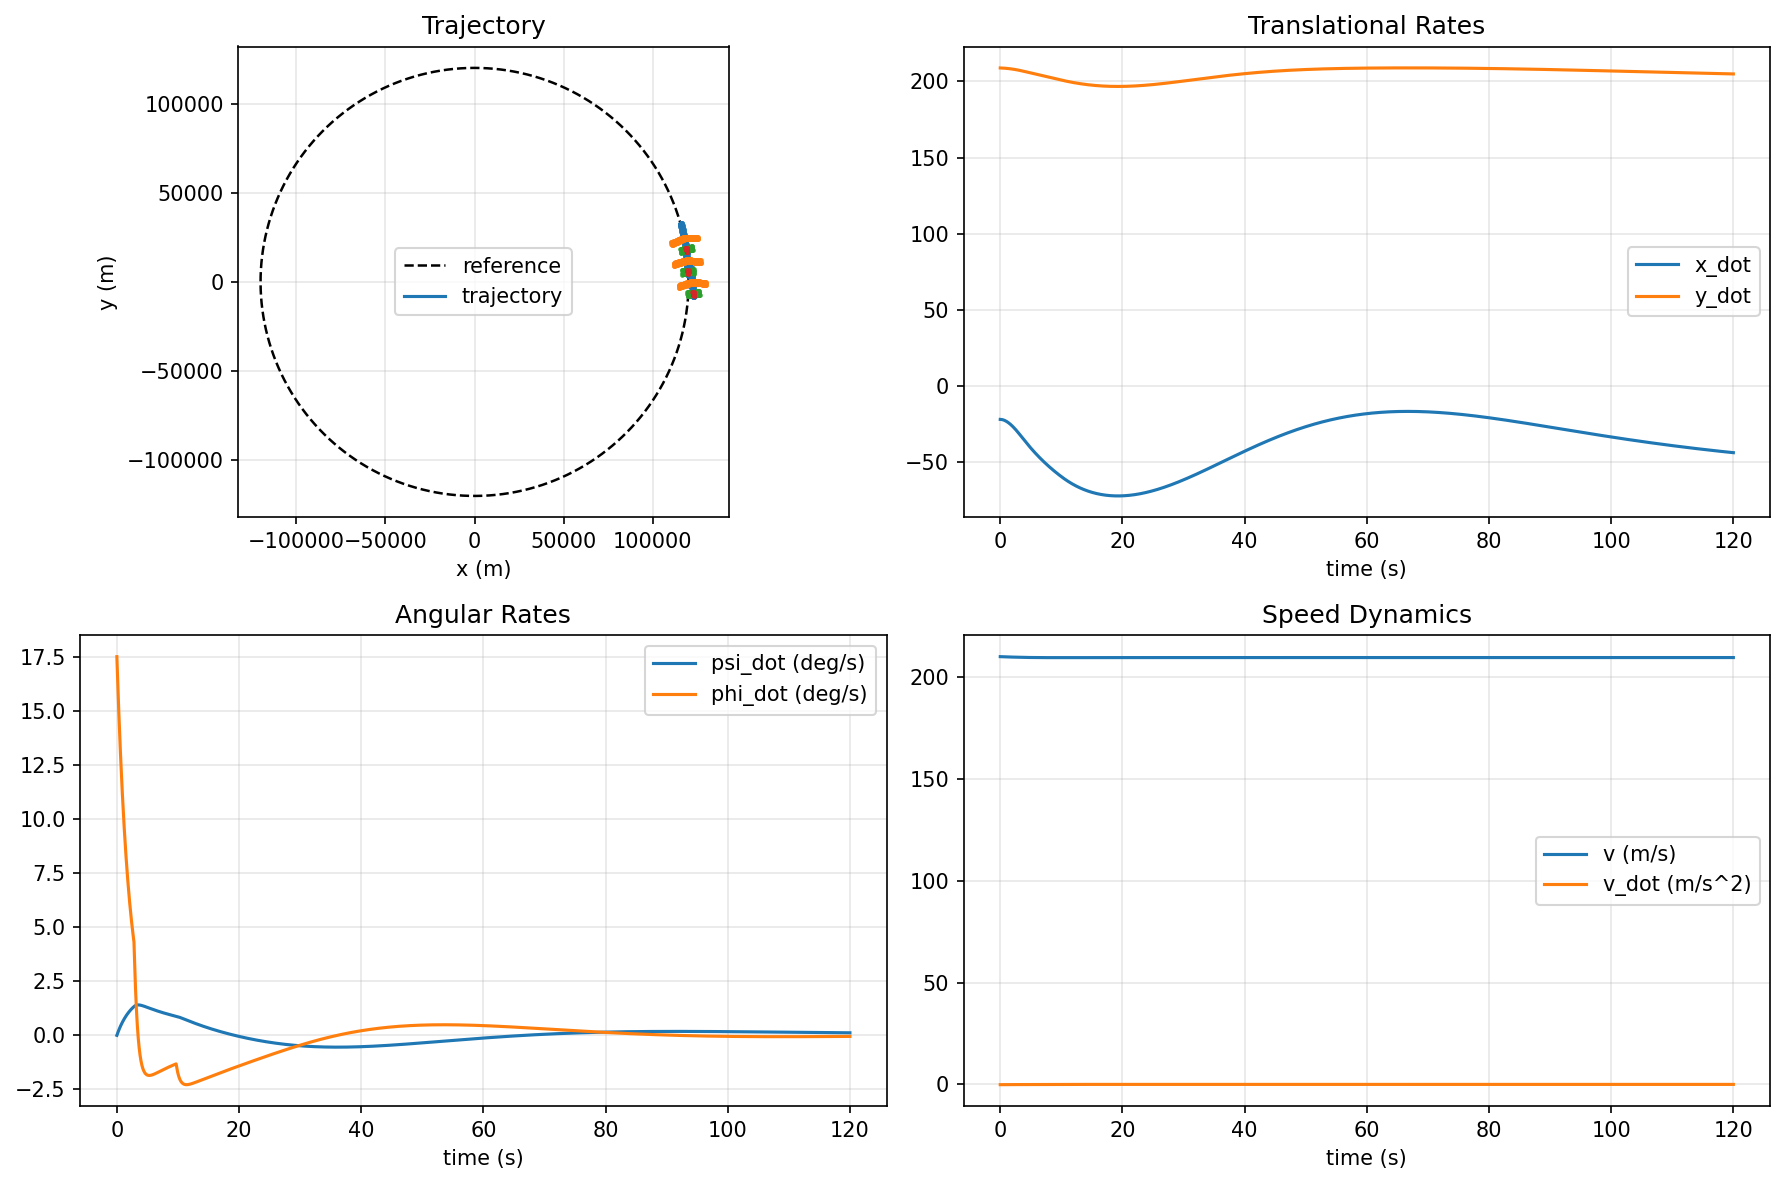
\includegraphics[width=0.93\textwidth]{assets/part2_dynamics.png}
\caption{Detailed dynamics figure: trajectory, translational rates, angular rates, and speed behavior.}
\label{fig:appendix-part2}
\end{figure}

Figure \ref{fig:appendix-part2} shows that the nominal trajectory follows the reference circle cleanly and that the translational, angular, and speed channels remain smooth throughout the maneuver.

\subsection{RK4/Euler Cross-Check}

The file \texttt{addicted/B747system.py} provides an independent benchmark for the same five-state planar model. It compares a fine-step RK4 reference with RK4 and Euler at \(\Delta t_{\mathrm{test}}=0.5\,\mathrm{s}\) under oscillatory bank input.

At \(t=100\,\mathrm{s}\), RK4 reduces the final state error norm from \(43.920\) to \(2.730\) and the mean error norm from \(28.479\) to \(2.250\). Although one isolated bank-angle error is not always smaller, the total state error and trajectory accuracy strongly favor RK4.

This external check supports the use of RK4 in \texttt{run.py} for nonlinear state propagation at practical step sizes.

\subsection{Transient Behavior in the First 120 Seconds}

Figure \ref{fig:transient-detail} isolates the first \(120\,\mathrm{s}\), where the aircraft removes the initial radial and angular offsets.

\begin{figure}[!htb]
\centering
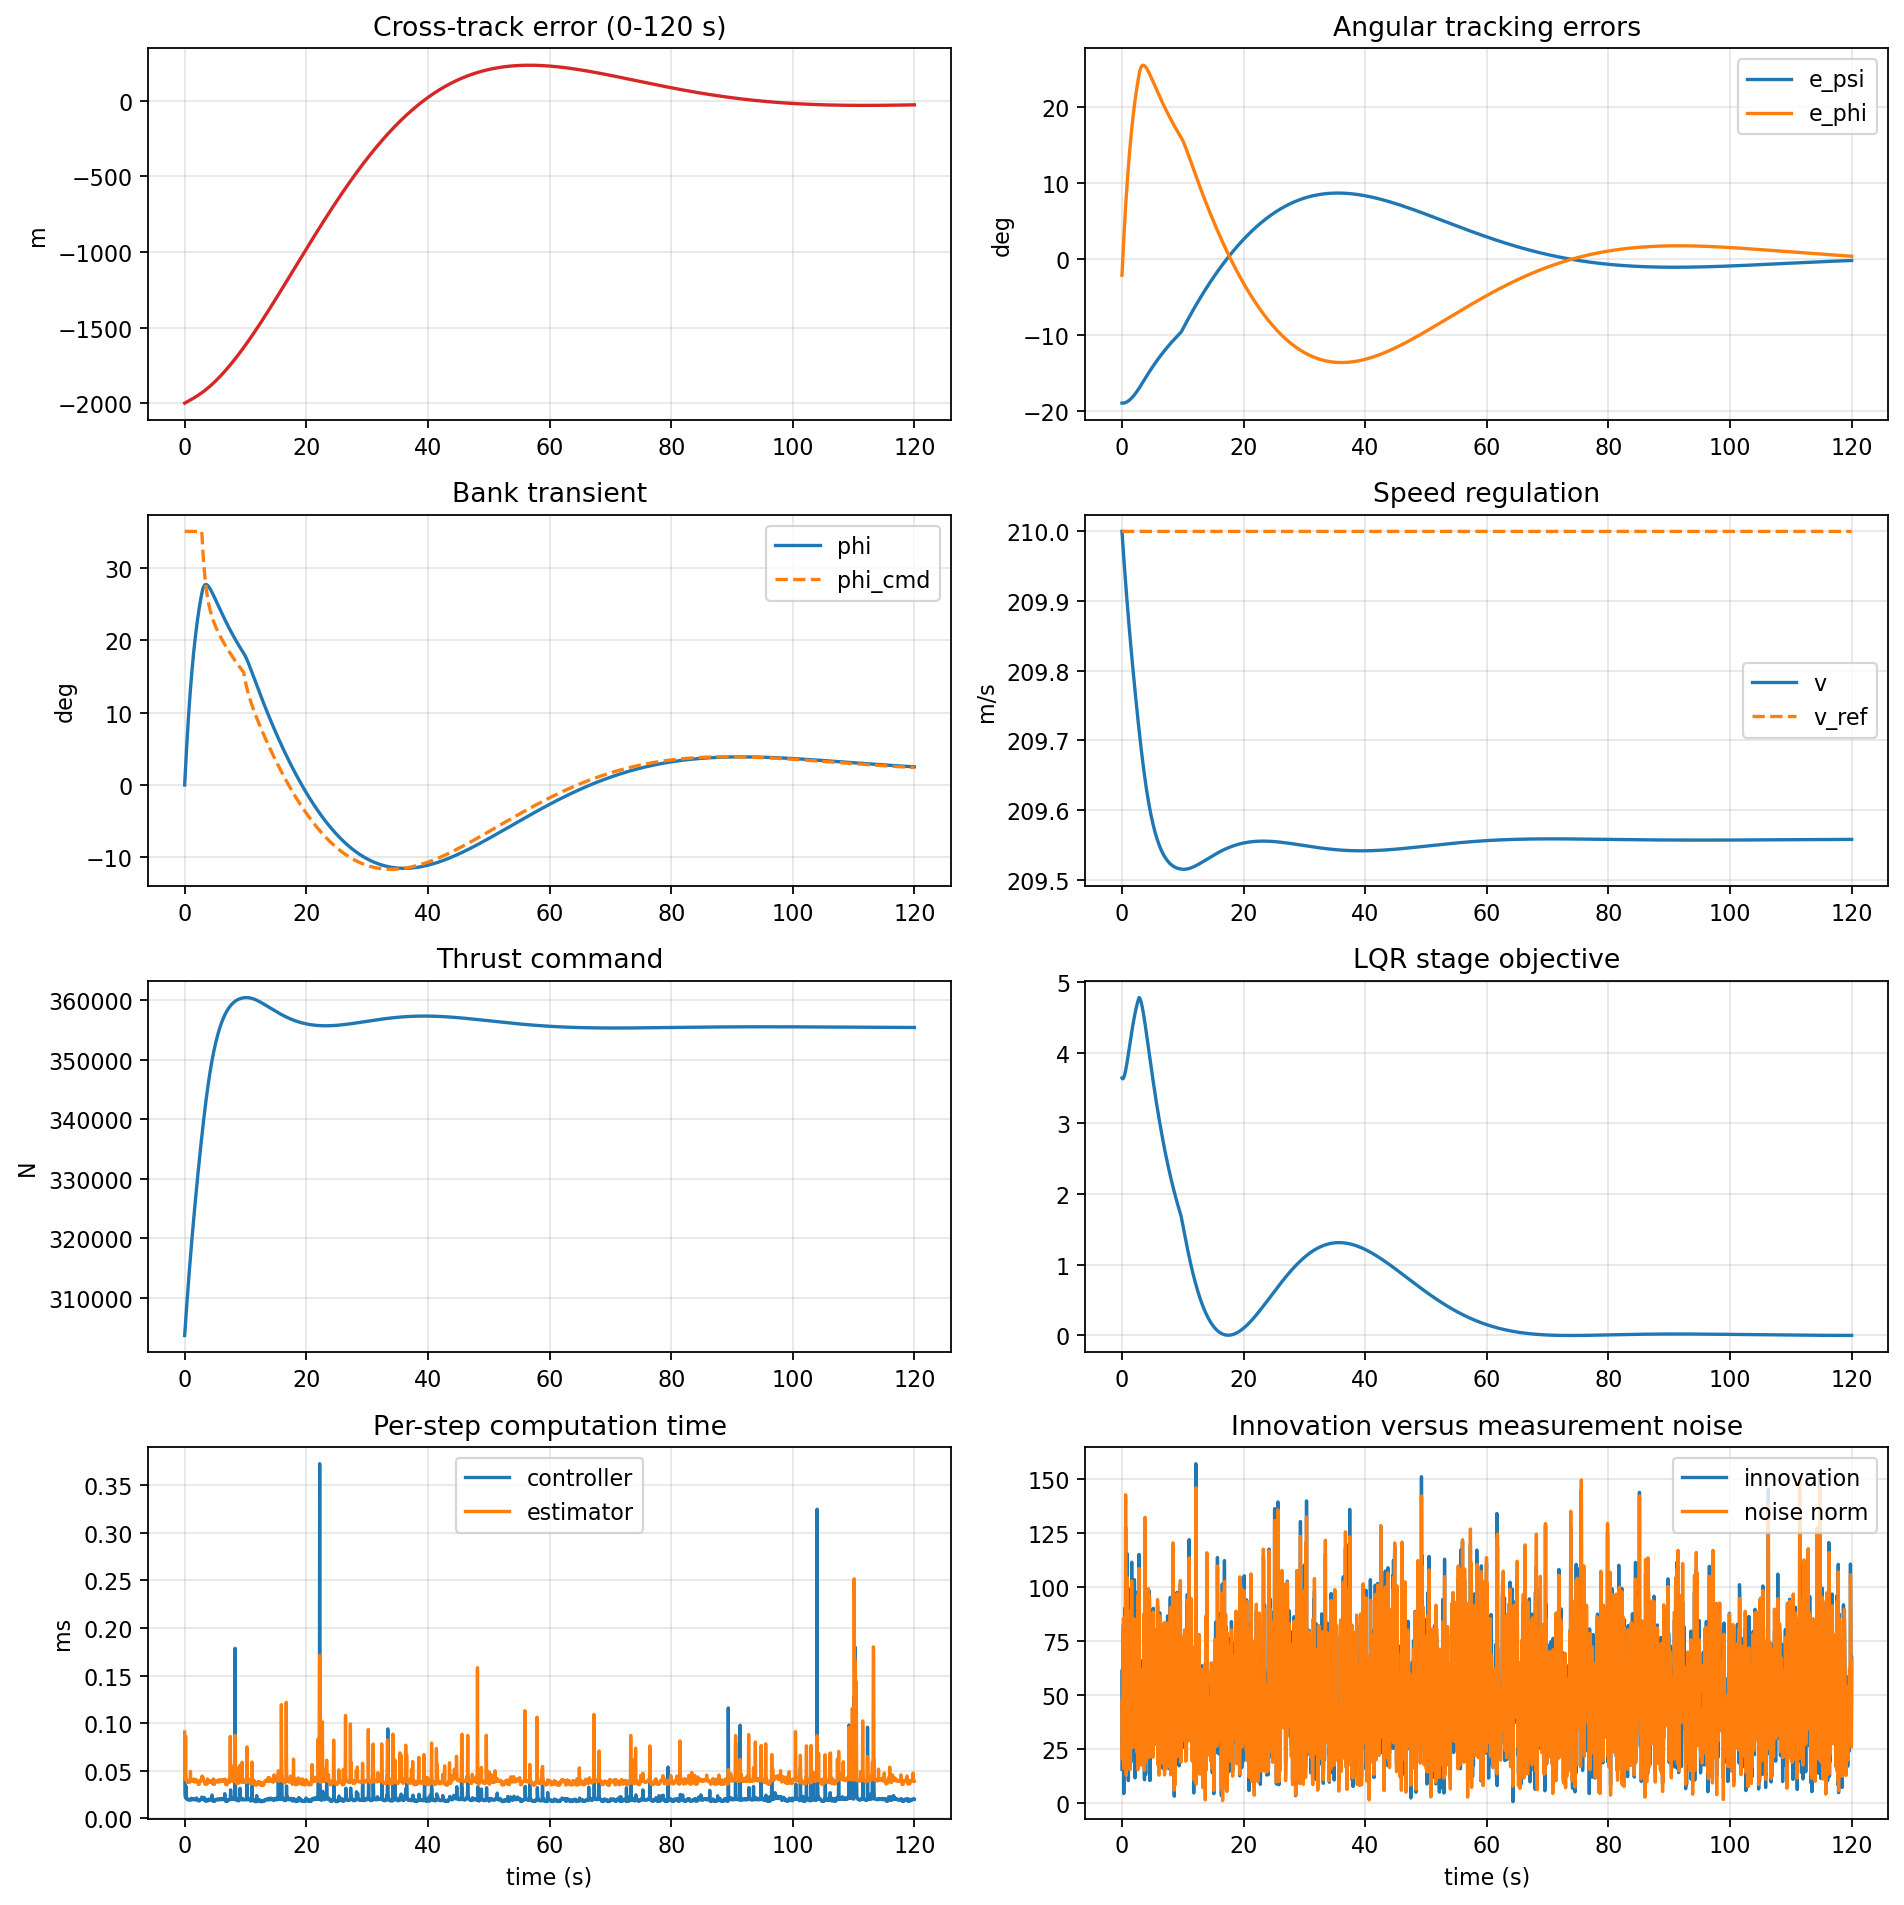
\includegraphics[width=0.96\textwidth]{assets/transient_detail.png}
\caption{Detailed transient response during the first 120 seconds of the baseline simulation.}
\label{fig:transient-detail}
\end{figure}

The transient is smooth: cross-track error decreases rapidly, bank angle follows the command with first-order lag, speed remains close to \(210\,\mathrm{m/s}\), and computation times stay negligible relative to the sampling interval.

\subsection{State-Estimation Consistency and Error Geometry}

Figure \ref{fig:state-estimate-comparison} compares each true state with its posterior estimate, while Figure \ref{fig:error-phase-hist} shows the controller error geometry and bank-angle distributions.

\begin{figure}[!htb]
\centering
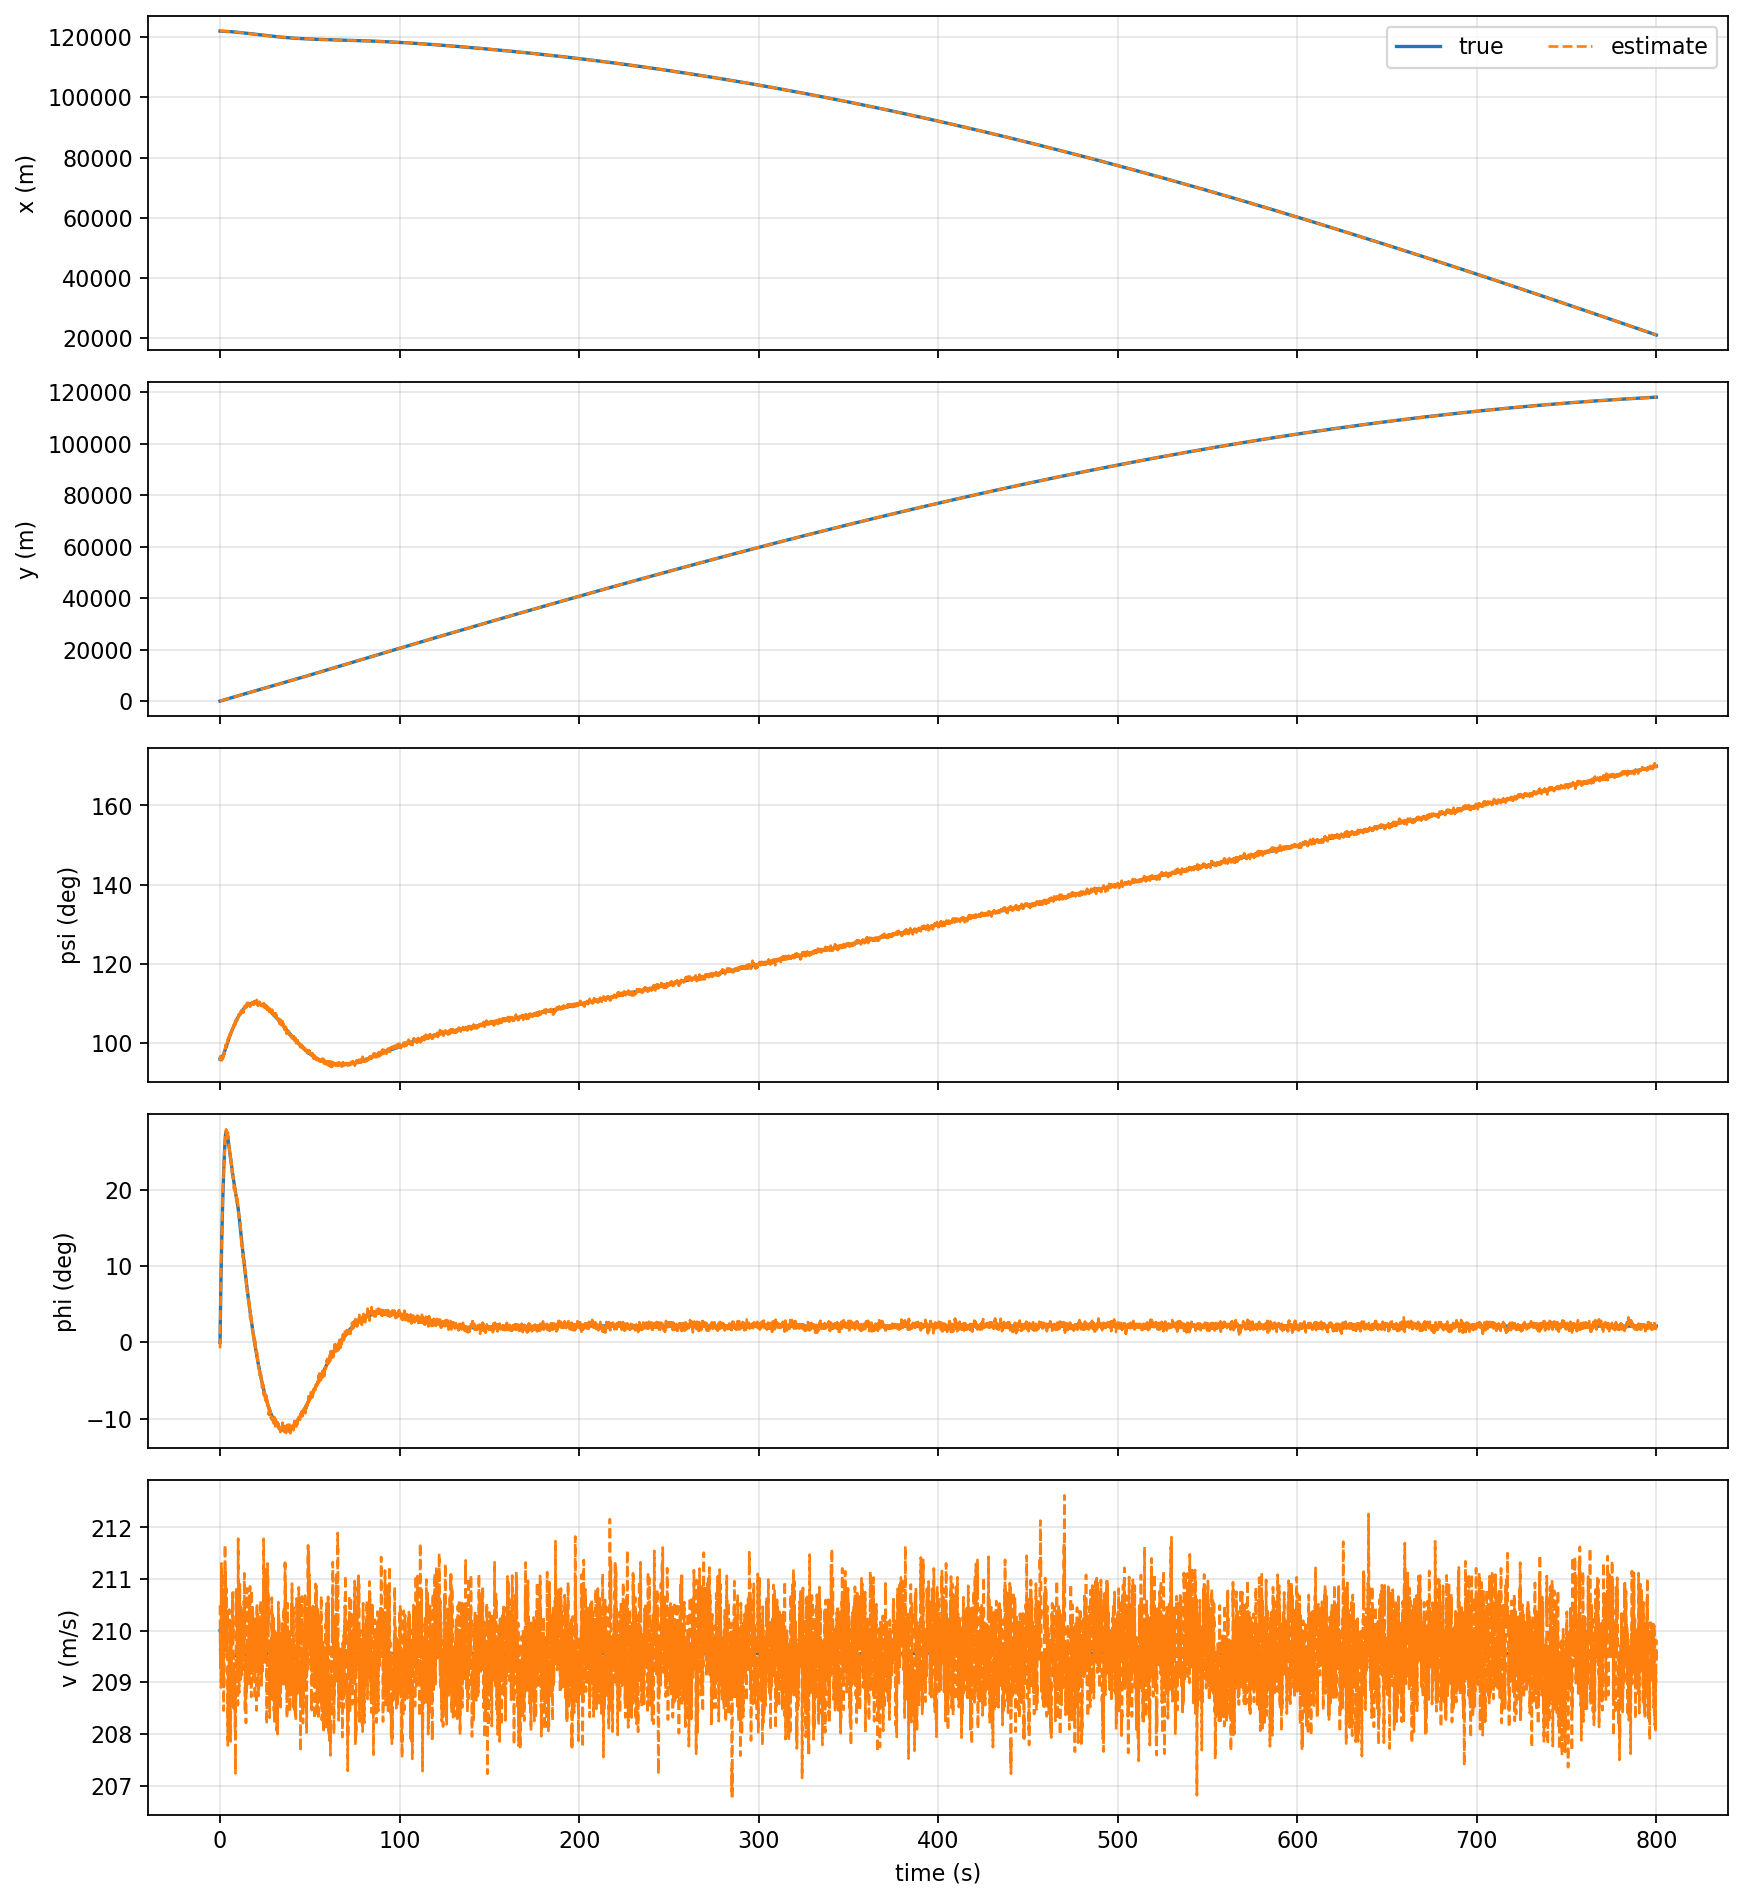
\includegraphics[width=0.93\textwidth]{assets/state_estimate_comparison.png}
\caption{True state and posterior estimate for all five state components.}
\label{fig:state-estimate-comparison}
\end{figure}

\begin{figure}[!htb]
\centering
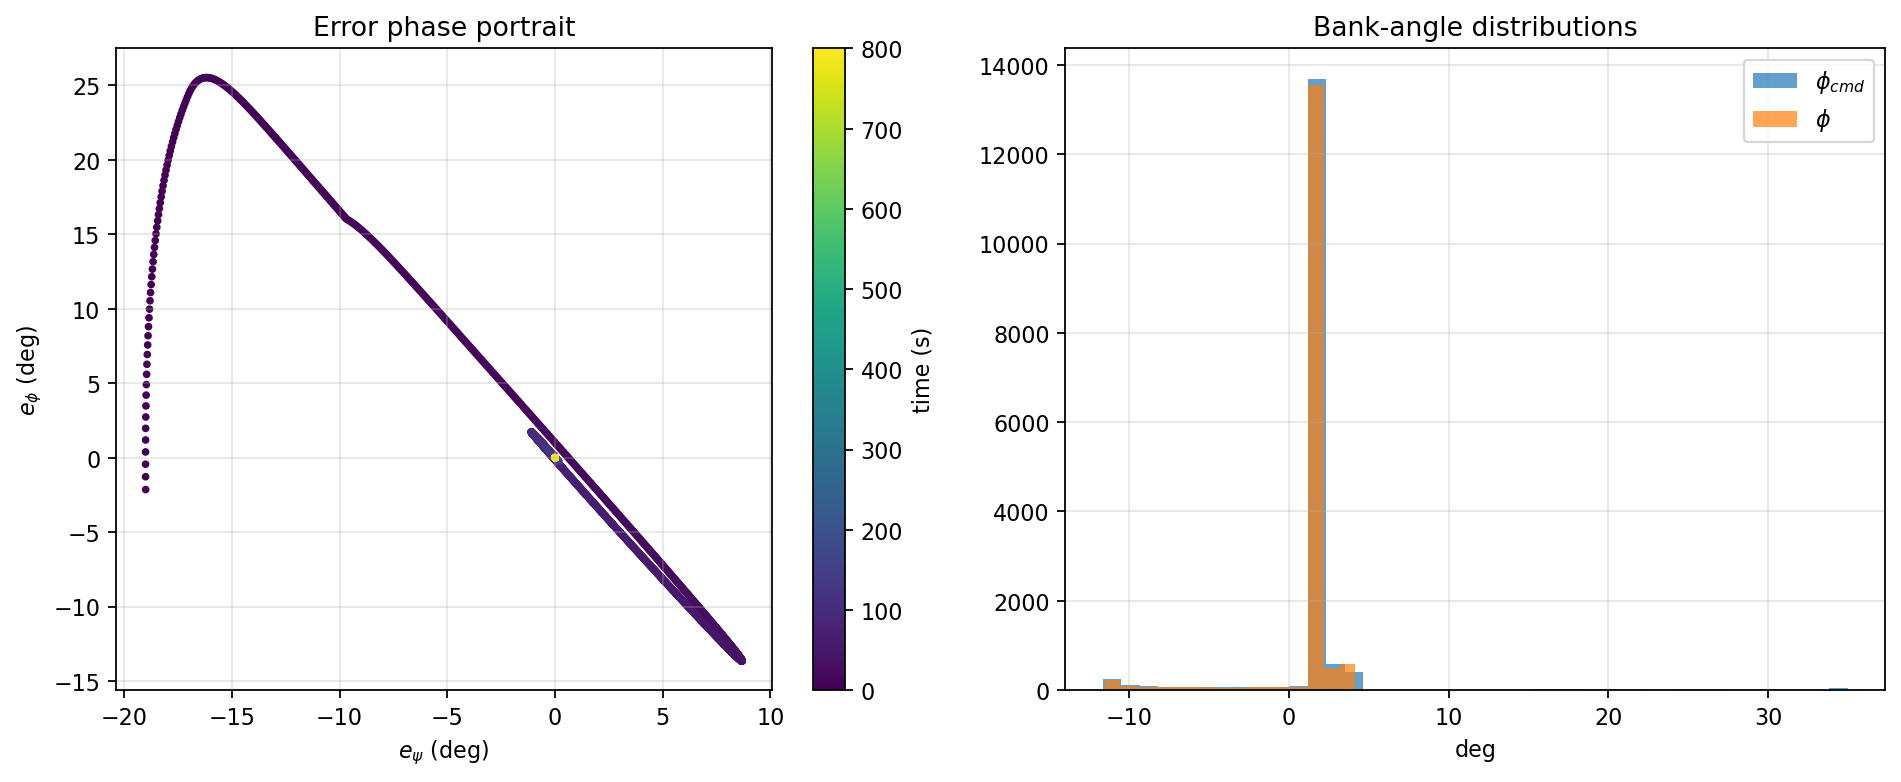
\includegraphics[width=0.93\textwidth]{assets/error_phase_and_hist.png}
\caption{Error phase portrait and bank-angle distributions in the baseline case.}
\label{fig:error-phase-hist}
\end{figure}

The true and estimated states remain close after the initial transient, consistent with the scalar estimation metrics reported earlier. The phase portrait also shows that the controller drives the joint error state toward the origin without large oscillatory loops.

\subsection{Sensitivity to Integration Time Step}

Figure \ref{fig:dt-sensitivity} compares closed-loop metrics for \(\Delta t=0.02, 0.05, 0.10,\) and \(0.20\,\mathrm{s}\) under otherwise identical settings.

\begin{figure}[!htb]
\centering
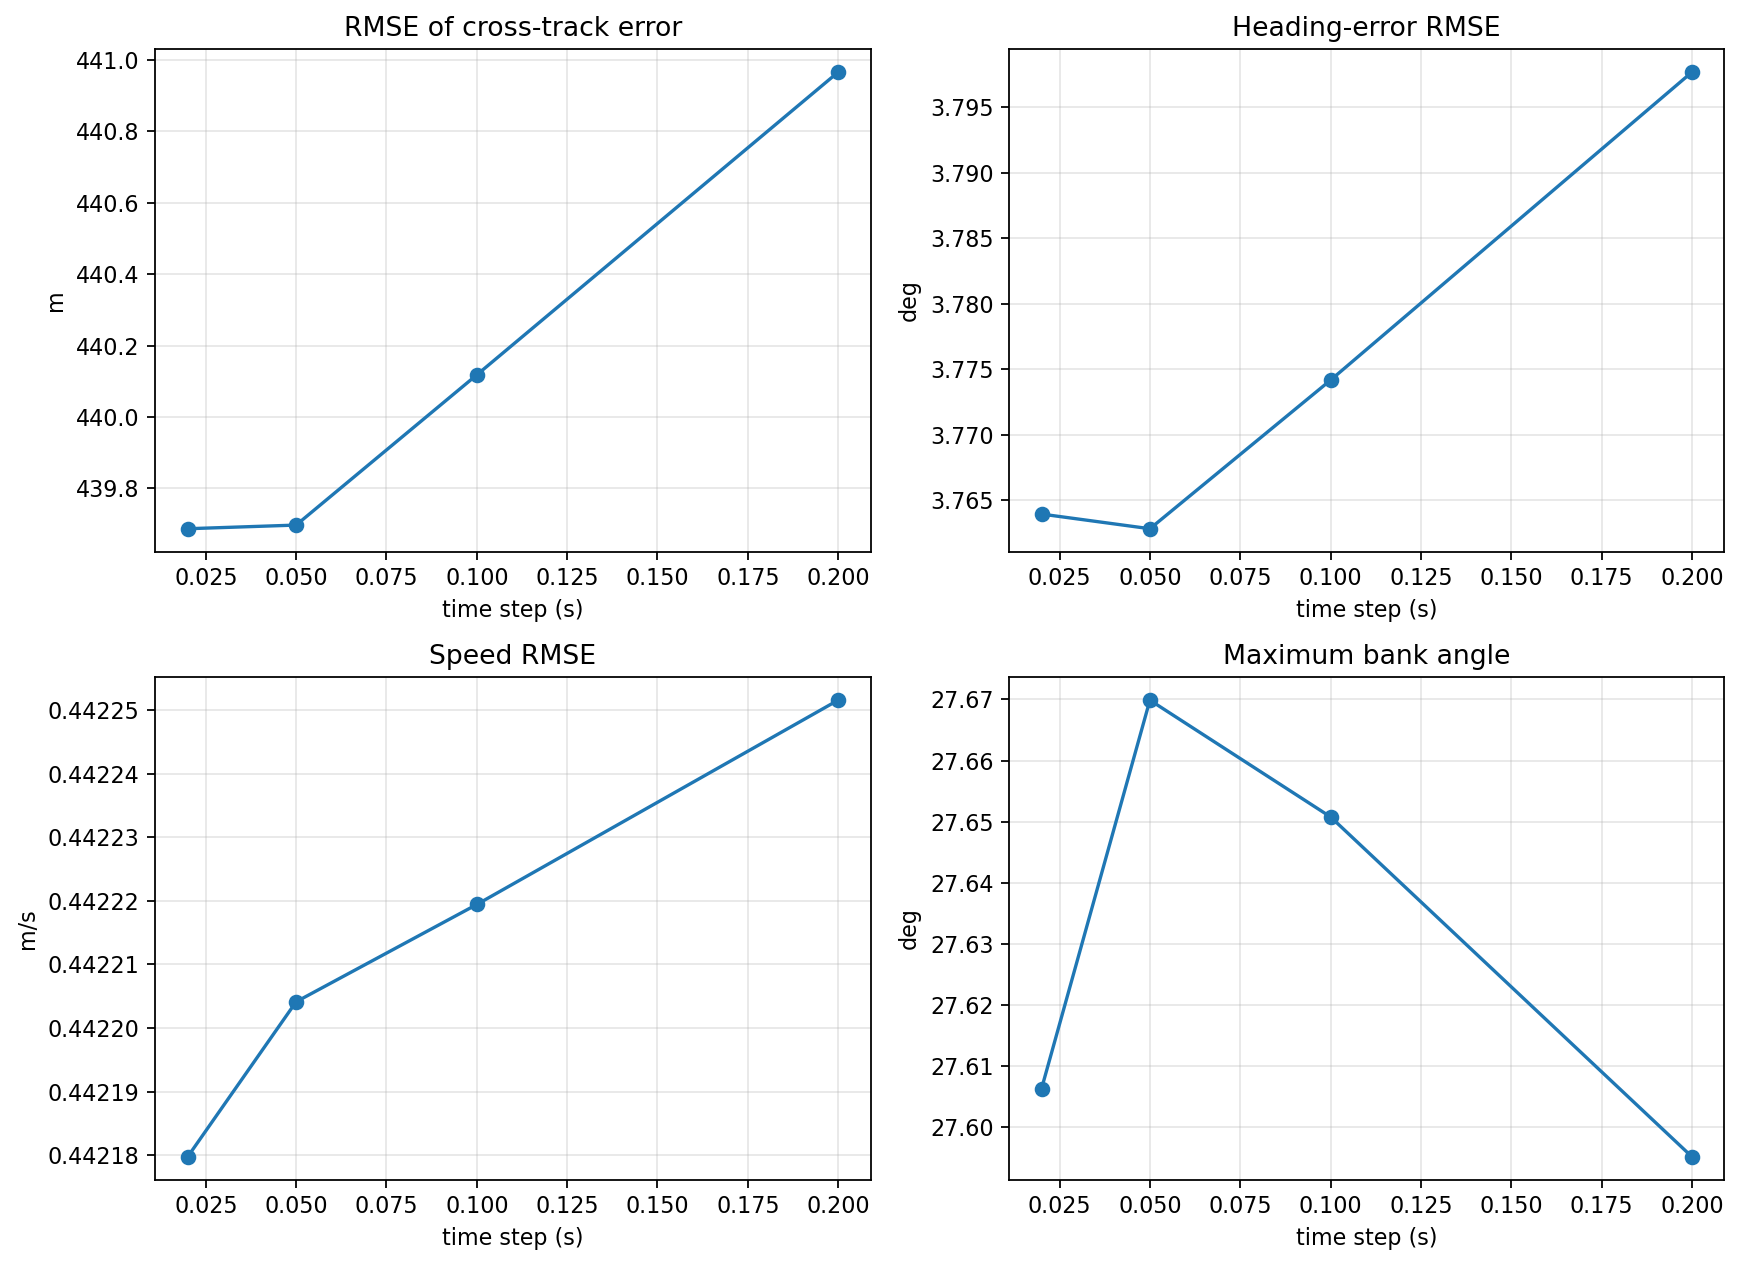
\includegraphics[width=0.92\textwidth]{assets/dt_sensitivity.png}
\caption{Sensitivity of tracking and regulation metrics to integration time step.}
\label{fig:dt-sensitivity}
\end{figure}

\begin{table}[!htb]
\centering
\caption{Selected metrics for the time-step sensitivity study}
\label{tab:dt-sensitivity}
\begin{tabular}{lrrrr}
\toprule
\(\Delta t\) (s) & RMSE(\(e_{ct}\)) (m) & Heading RMSE (deg) & Speed RMSE (m/s) & Max \(|\phi|\) (deg) \\
\midrule
0.02 & 439.63 & 3.77 & 0.2762 & 27.61 \\
0.05 & 439.64 & 3.76 & 0.2762 & 27.67 \\
0.10 & 440.06 & 3.78 & 0.2762 & 27.65 \\
0.20 & 440.91 & 3.80 & 0.2762 & 27.60 \\
\bottomrule
\end{tabular}
\end{table}

Table \ref{tab:dt-sensitivity} and Figure \ref{fig:dt-sensitivity} show only mild variation across the tested step sizes. The baseline choice \(\Delta t=0.05\,\mathrm{s}\) is therefore sufficiently conservative for stable and accurate closed-loop simulation.

\subsection{Sensitivity to Reference-Circle Radius}

Figure \ref{fig:radius-sensitivity} compares four reference radii between \(80{,}000\,\mathrm{m}\) and \(200{,}000\,\mathrm{m}\).

\begin{figure}[!htb]
\centering
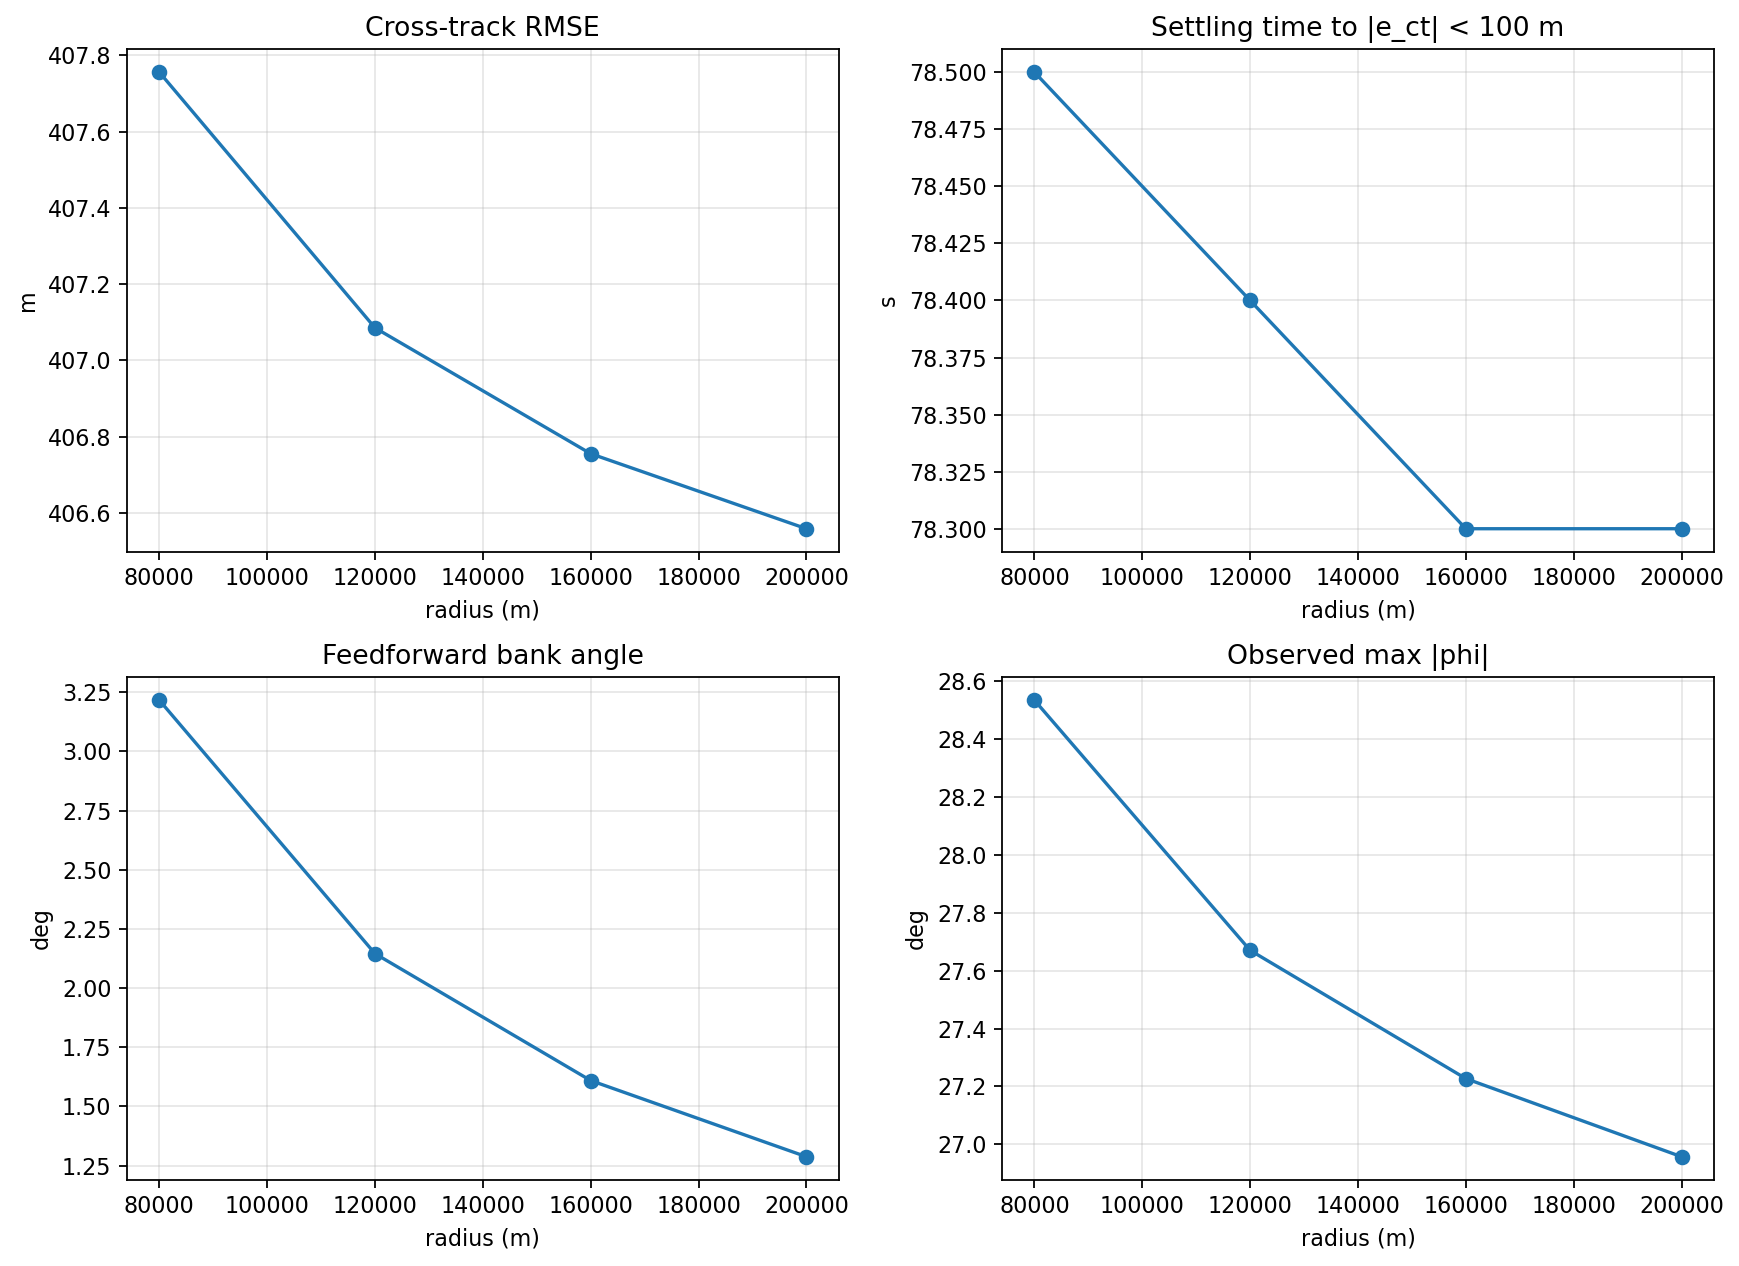
\includegraphics[width=0.92\textwidth]{assets/radius_sensitivity.png}
\caption{Sensitivity of performance and commanded curvature to reference-circle radius.}
\label{fig:radius-sensitivity}
\end{figure}

As the radius increases, the feedforward and observed bank angles decrease monotonically, while tracking RMSE changes only modestly. The controller therefore generalizes well across a useful range of path curvatures.

\begin{figure}[!htb]
\centering
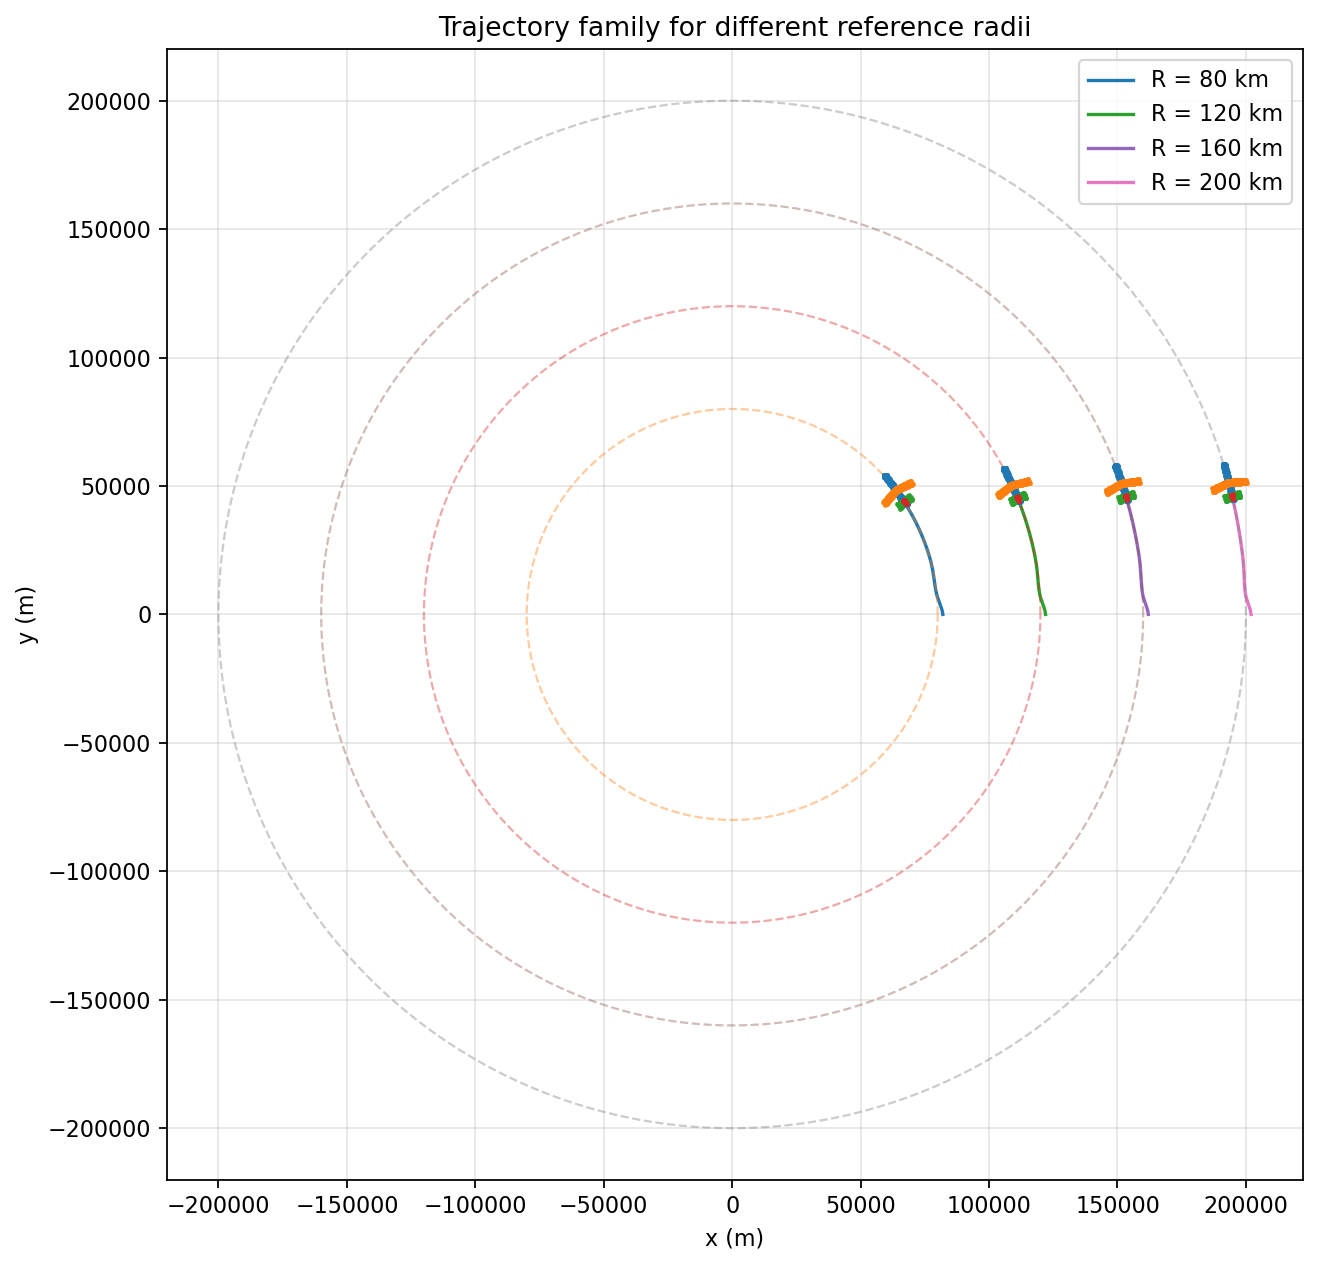
\includegraphics[width=0.93\textwidth]{assets/trajectory_family.png}
\caption{Family of closed-loop trajectories under different reference-circle radii.}
\label{fig:trajectory-family}
\end{figure}

Figure \ref{fig:trajectory-family} shows that all tested cases converge toward their respective circles without pathological behavior.

\subsection{Sensitivity to Measurement Noise}

Figure \ref{fig:noise-sensitivity} scales the measurement-noise covariance from \(0.5\) to \(4.0\) times the baseline value.

\begin{figure}[!htb]
\centering
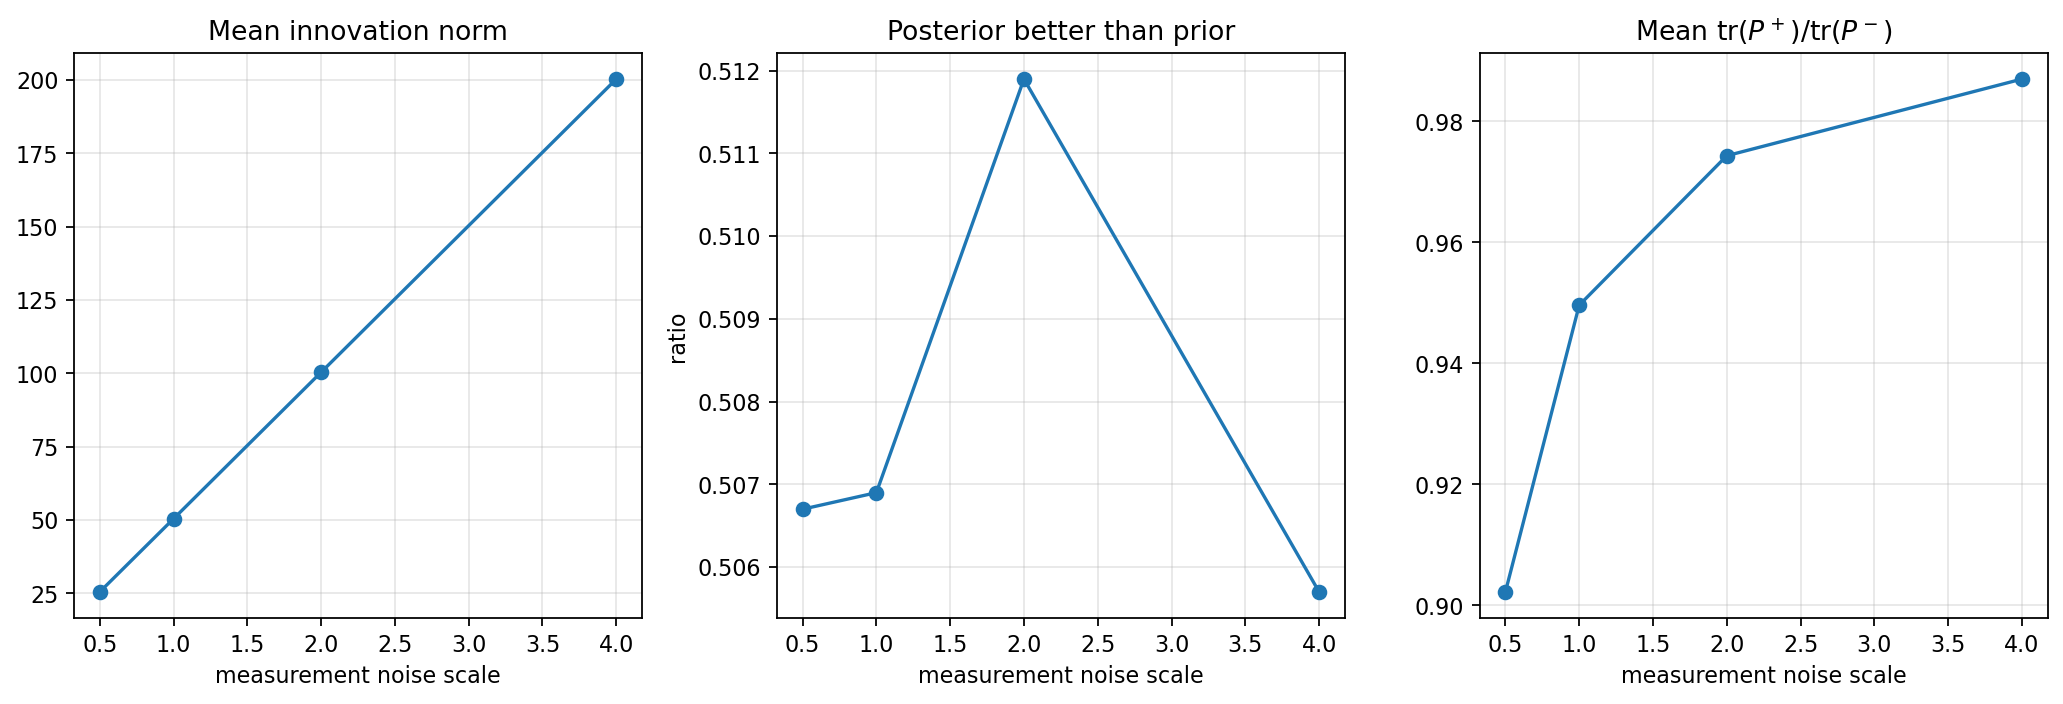
\includegraphics[width=0.92\textwidth]{assets/noise_sensitivity.png}
\caption{Estimator sensitivity to measurement-noise scaling.}
\label{fig:noise-sensitivity}
\end{figure}

Tracking metrics remain nearly unchanged because control does not yet use the estimate, whereas estimation errors and innovation norms increase clearly with noise level. The sweep therefore isolates estimator sensitivity without confounding it with controller behavior.

\subsection{Sensitivity to LQR Weight Selection}

Figure \ref{fig:lqr-weight-sensitivity} compares conservative, baseline, and aggressive LQR weights.

\begin{figure}[!htb]
\centering
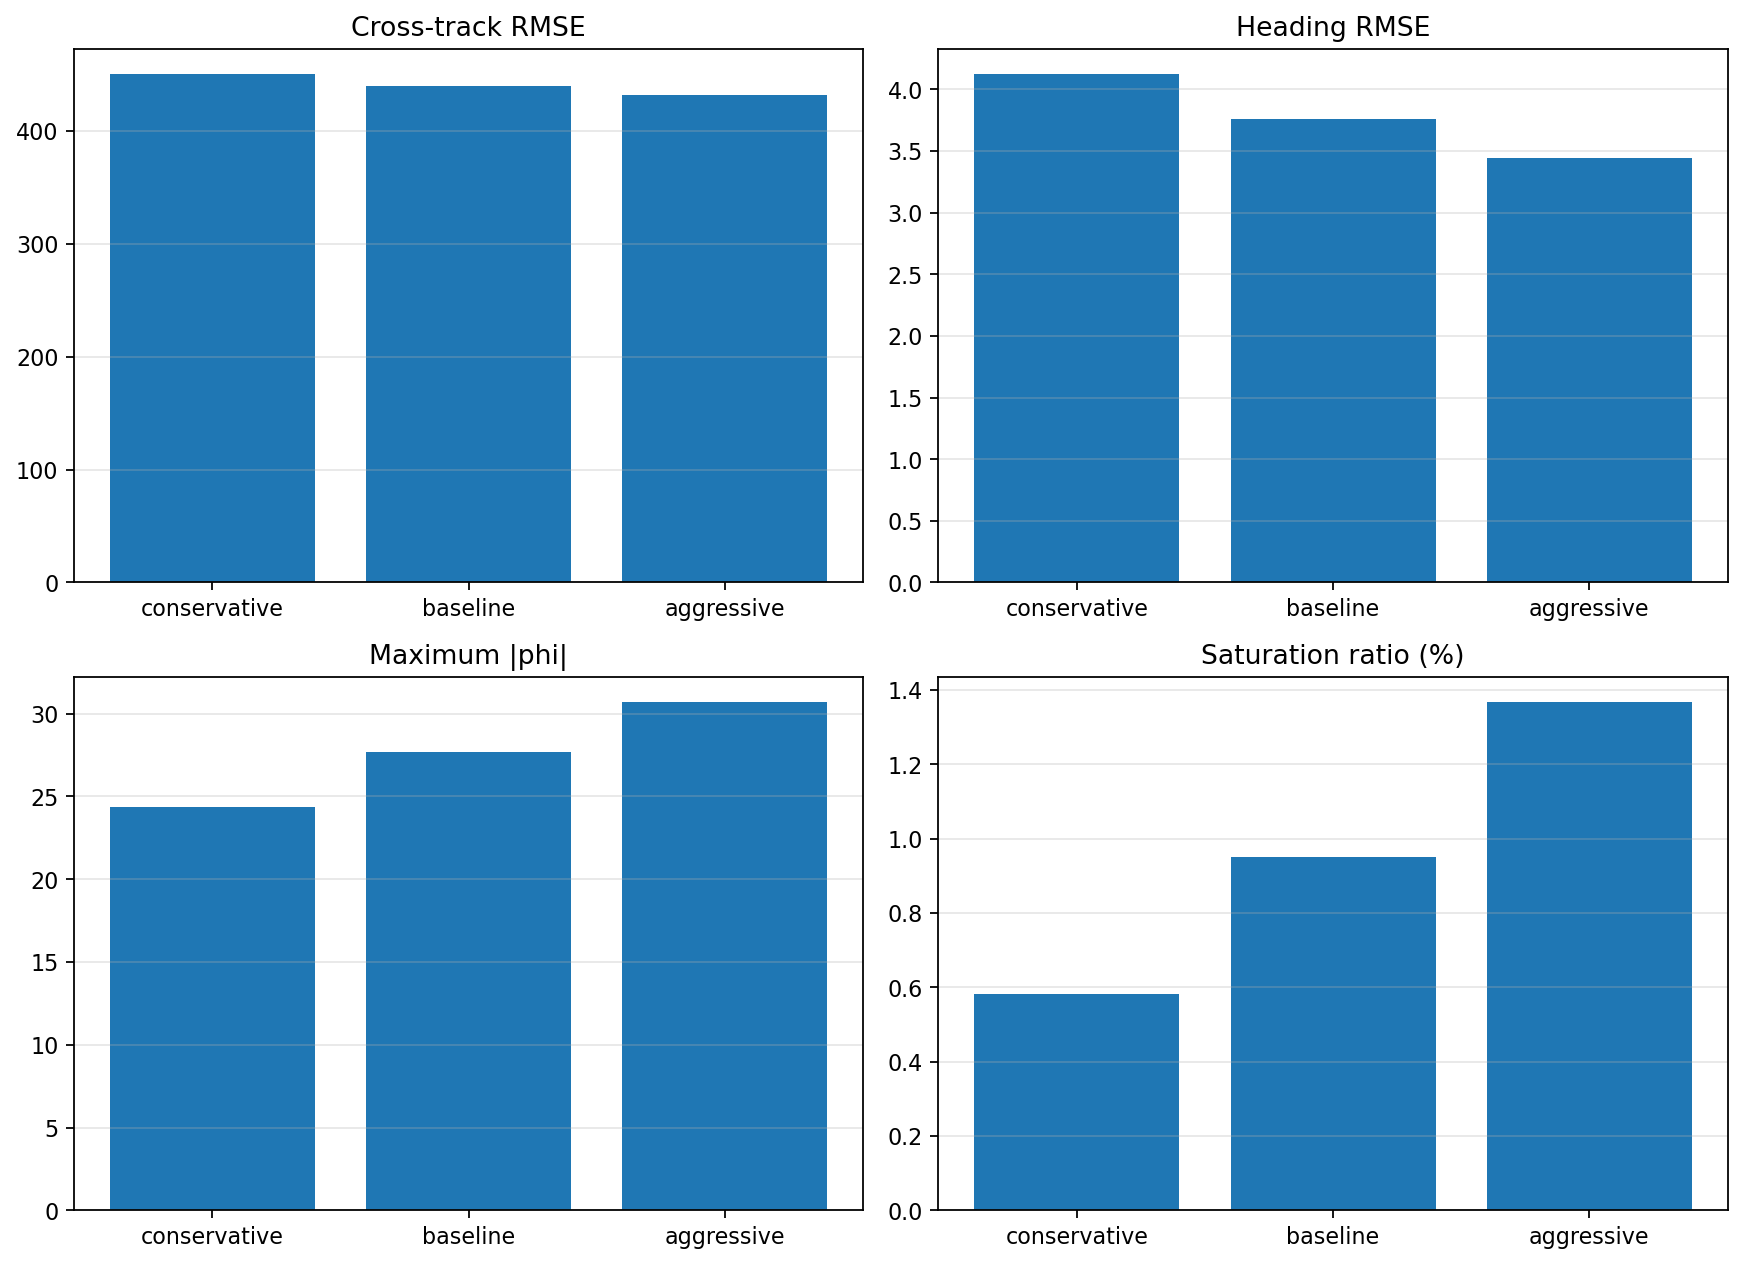
\includegraphics[width=0.92\textwidth]{assets/lqr_weight_sensitivity.png}
\caption{Effect of LQR weight selection on tracking quality and actuator usage.}
\label{fig:lqr-weight-sensitivity}
\end{figure}

The aggressive design improves tracking but increases peak bank angle and saturation, whereas the conservative design reduces control effort at the expense of weaker correction. The baseline choice remains the best compromise between responsiveness and actuator margin.

\subsection{Recreated RK4-versus-Euler Benchmark}

Figure \ref{fig:rk4-vs-euler-project} recreates the supplementary RK4/Euler benchmark using the project dynamics implementation.

\begin{figure}[!htb]
\centering
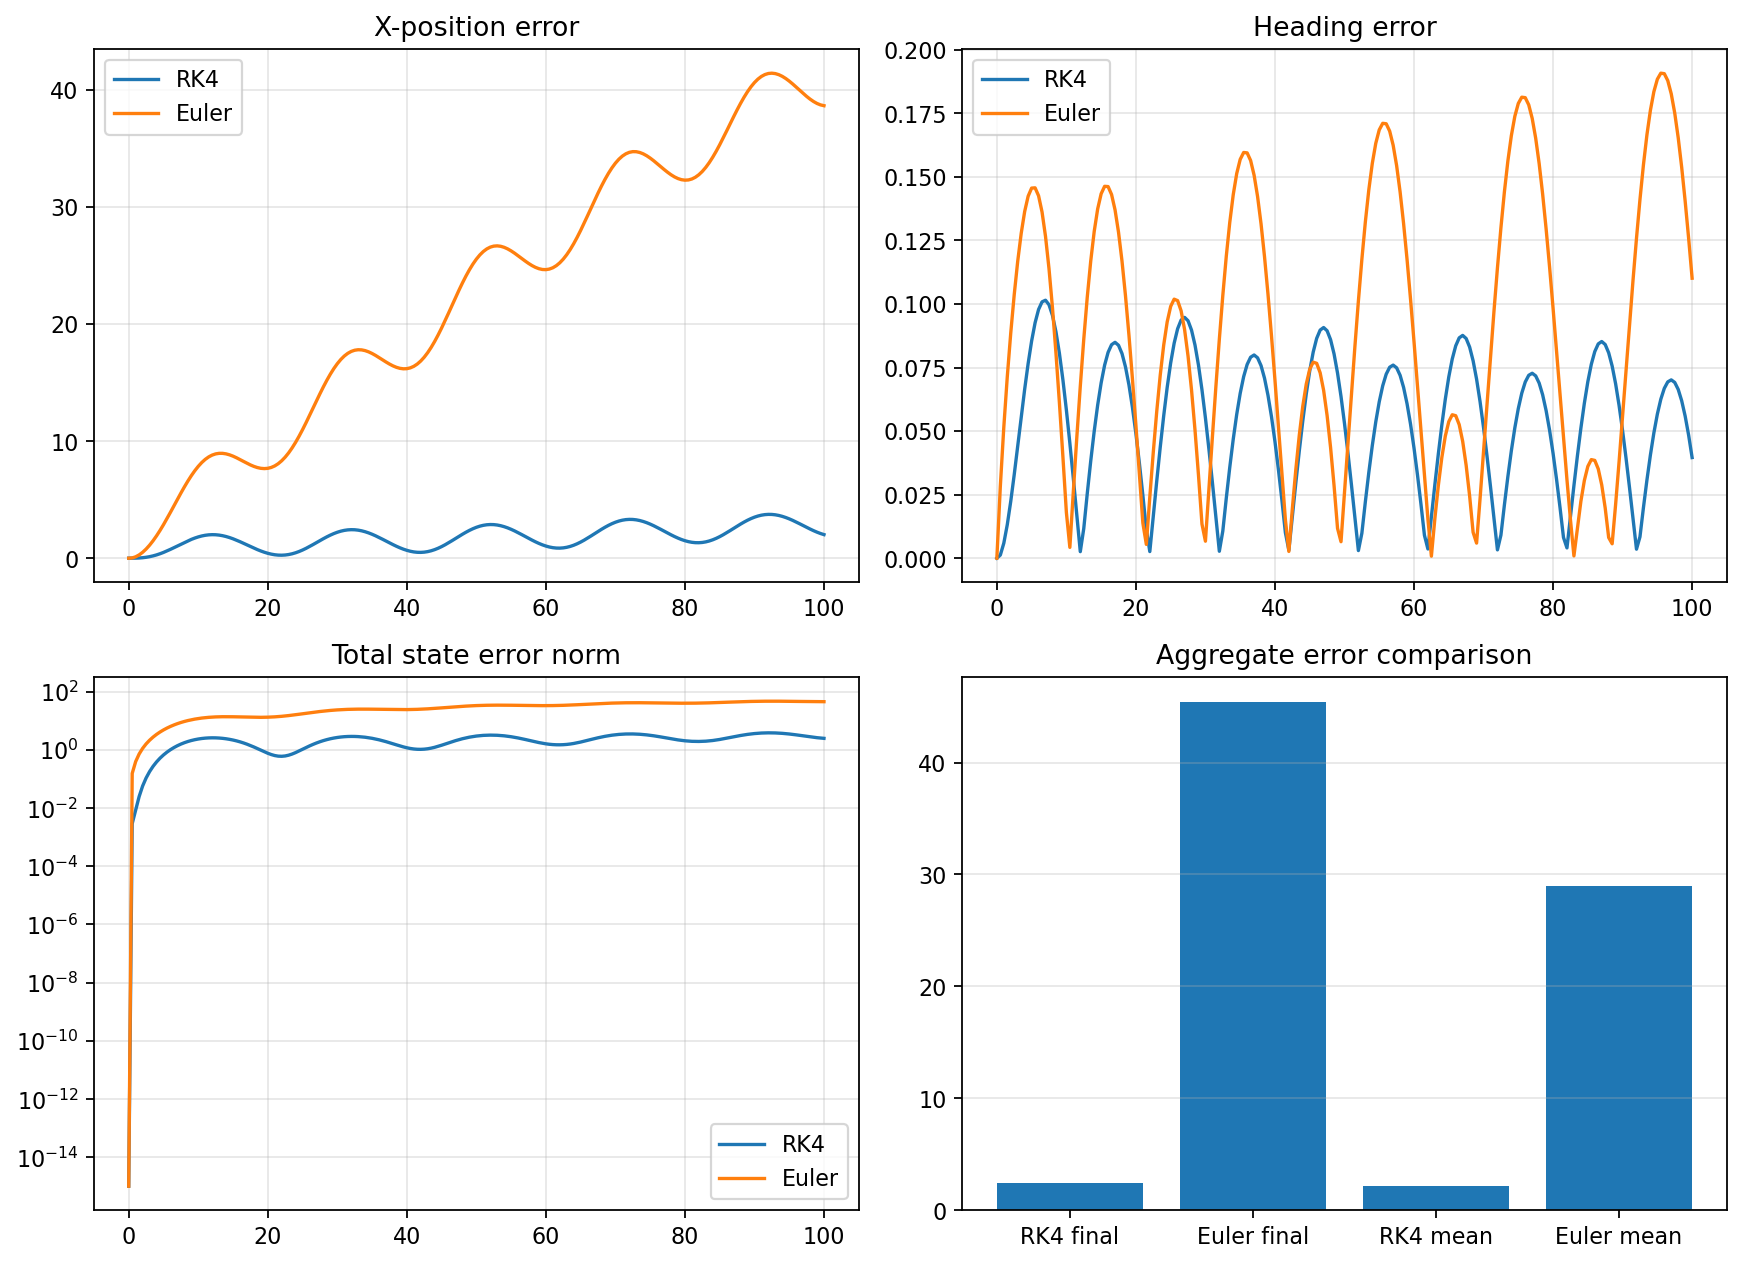
\includegraphics[width=0.93\textwidth]{assets/rk4_vs_euler_project.png}
\caption{Recreated RK4-versus-Euler benchmark using the project dynamics implementation.}
\label{fig:rk4-vs-euler-project}
\end{figure}

The recreated benchmark matches the independent script closely: RK4 is about \(16.46\times\) better than Euler in final total state error and about \(12.68\times\) better in mean total state error. This consistency reinforces the numerical advantage of RK4 for the present nonlinear dynamics model.

\section{Discussion}

The combined results show that the controller-estimator architecture is stable, computationally light, and accurate enough for circular tracking in the present nonlinear planar model. Outer-loop geometric correction removes large radial offsets effectively, inner-loop LQR regulates heading and bank dynamics well, and RK4 keeps propagation error from dominating the closed-loop response.

The framework nevertheless remains simplified. The aircraft model is planar, the LQR design uses a first-order discretization, and the estimator is not yet closed around the controller. These assumptions are acceptable for coursework demonstration but limit physical fidelity and robustness claims.

Future work could close the loop around estimated states, incorporate disturbances such as wind, and extend the design toward uncertainty-aware formulations including stochastic, robust, and distributionally robust optimization \supercite{birge1997,haneveld2020,bental2009,bertsimas2011,blanchet2024,bomze2022}.

\section{Conclusion}

This project successfully demonstrates an integrated Boeing 747 circular-tracking simulation pipeline. LQR provides stable and accurate inner-loop regulation, RK4 supplies reliable nonlinear state propagation, and Gaussian Bayes/MAP estimation offers interpretable uncertainty diagnostics. Under the default configuration, the system reaches very small steady-state cross-track and speed errors while respecting actuator limits.

The main limitations are the planar flight assumption, simplified actuator and disturbance modeling, first-order discretization in LQR design, and the use of true state rather than estimated state for feedback. Future work should close the loop around estimated states, include wind and disturbance models, compare against alternative controllers such as MPC or nonlinear guidance laws, and extend the system to higher-fidelity aircraft dynamics.

\section{One-Page Summary of Group Contributions}


\begin{table}[!htb]
\centering
\caption{Group contribution summary}
\small
\setlength{\tabcolsep}{4pt}
\begin{adjustbox}{max width=\textwidth}
\begin{tabular}{>{\raggedright\arraybackslash}p{0.16\textwidth} >{\raggedright\arraybackslash}p{0.15\textwidth} >{\raggedright\arraybackslash}p{0.23\textwidth} >{\raggedright\arraybackslash}p{0.23\textwidth} >{\centering\arraybackslash}p{0.13\textwidth}}
\toprule
Group Member & Student ID & Specific Components & Deliverables / Evidence & Overall Contribution (\%) \\
\midrule
Yufa You & 25144639R & Topic selection, coding, algorithm design, report writing & Core project implementation, algorithm development, and report drafting & 50 \\
Ruige Yang & 25145125R & Formula derivation, experimental result organization, presentation preparation & Analytical derivations, result curation, and presentation materials & 50 \\
\bottomrule
\end{tabular}
\end{adjustbox}
\end{table}


Yufa You led topic selection, implemented the main codebase, designed the core algorithms, and wrote the report. Ruige Yang focused on formula derivation, organization of the experimental results, and preparation of the presentation materials. Both members jointly reviewed the final manuscript and checked the consistency of the submitted outputs.

%TC:ignore
\singlespacing
\emergencystretch 3em
\hfuzz 1px
\printbibliography[heading=bibnumbered]
%TC:endignore
\end{document}
